\documentclass{ximera}

%
%%% Begin Laad packages
%
\makeatletter
\@ifclassloaded{xourse}{%
    \typeout{Start loading preamble.tex (in a XOURSE)}%
    \def\isXourse{true}   % automatically defined; pre 112022 it had to be set 'manually' in a xourse
}{%
    \typeout{Start loading preamble.tex (NOT in a XOURSE)}%
}
\makeatother

\pgfplotsset{compat=1.16}

\usepackage{currfile}

% 201908/202301: PAS OP: babel en doclicense lijken problemen te veroorzaken in .jax bestand
% (wegens syntax error met toegevoegde \newcommands ...)
\pdfOnly{
    \usepackage[hyperxmp=false,type={CC},modifier={by-nc-sa},version={4.0}]{doclicense}
    \usepackage[dutch]{babel}
}


\usepackage[utf8]{inputenc}
\usepackage{morewrites}   % nav zomercursus (answer...?)
\usepackage{multirow}
\usepackage{multicol}
\usepackage{tikzsymbols}
\usepackage{tikz-3dplot}
\usepackage{ifthen}
%\usepackage{animate} BREAKS HTML STRUCTURE USED BY XIMERA
\usepackage{relsize}

\usepackage{eurosym}    % \euro  (€ werkt niet in xake ...?)
\usepackage{wrapfig}

\usepackage{cancel}

\usepackage{tabularx}
% Nuttig als ook interactieve beamer slides worden voorzien:
\providecommand{\p}{} % default nothing ; potentially usefull for slides: redefine as \pause
%providecommand{\p}{\pause}

\usepackage{caption} % captionof
%\usepackage{pdflscape}    % landscape environment

% Met "\newcommand\showtodonotes{}" kan je todonotes tonen (in pdf/online)
% 201908: online werkt het niet (goed)
\providecommand\showtodonotes{disable}
\providecommand\todo[1]{\typeout{TODO #1}}
%\usepackage[\showtodonotes]{todonotes}
%\usepackage{todonotes}

%
% Poging tot aanpassen layout
%
\usepackage{tcolorbox}
\tcbuselibrary{theorems}

%%% Einde laad packages

%%% Begin Ximera specifieke zaken

% \graphicspath{
% 	{../../}
% 	{../}
% 	{./}
%   	{../../pictures/}
%    	{../pictures/}
%    	{./pictures/}
% 	{./explog/}    % M05 in groeimodellen       
% }

%%% Einde Ximera specifieke zaken

%
% define softer blue/red/green, use KU Leuven base colors for blue (and dark orange for red ?)
%
% todo: rather redefine blue/red/green ...?
%\definecolor{xmblue}{rgb}{0.01, 0.31, 0.59}
%\definecolor{xmred}{rgb}{0.89, 0.02, 0.17}
\definecolor{xmdarkblue}{rgb}{0.122, 0.671, 0.835}   % KU Leuven Blauw
\definecolor{xmblue}{rgb}{0.114, 0.553, 0.69}        % KU Leuven Blauw
\definecolor{xmgreen}{rgb}{0.13, 0.55, 0.13}         % No KULeuven variant for green found ...

\definecolor{xmaccent}{rgb}{0.867, 0.541, 0.18}      % KU Leuven Accent (orange ...)
\definecolor{kuaccent}{rgb}{0.867, 0.541, 0.18}      % KU Leuven Accent (orange ...)

\colorlet{xmred}{xmaccent!50!black}                  % Darker version of KU Leuven Accent

\providecommand{\blue}[1]{{\color{blue}#1}}    
\providecommand{\red}[1]{{\color{red}#1}}

\renewcommand\CancelColor{\color{xmaccent!50!black}}

% werkt in math en text mode om MATH met oranje (of grijze...)  achtergond te tonen (ook \important{\text{blabla}} lijkt te werken)
%\newcommand{\important}[1]{\ensuremath{\colorbox{xmaccent!50!white}{$#1$}}}   % werkt niet in Mathjax
%\newcommand{\important}[1]{\ensuremath{\colorbox{lightgray}{$#1$}}}
%\newcommand{\important}[1]{\ensuremath{\colorbox{orange}{$#1$}}}   % TODO: kleur aanpassen voor mathjax; wordt overschreven infra!
\newcommand{\important}[1]{\ensuremath{\fcolorbox{black}{white}{$#1$}}}


% Uitzonderlijk kan met \pdfnl in de PDF een newline worden geforceerd, die online niet nodig/nuttig is omdat daar de regellengte hoe dan ook niet gekend is.
\ifdefined\HCode%
\providecommand{\pdfnl}{}%
\else%
\providecommand{\pdfnl}{%
  \\%
}%
\fi

% Uitzonderlijk kan met \handoutnl in de handout-PDF een newline worden geforceerd, die noch online noch in de PDF-met-antwoorden nuttig is.
\ifdefined\HCode
\providecommand{\handoutnl}{}
\else
\providecommand{\handoutnl}{%
\ifhandout%
  \nl%
\fi%
}
\fi



% \cellcolor IGNORED by tex4ht ?
% \begin{center} seems not to wordk
    % (missing margin-left: auto;   on tabular-inside-center ???)
%\newcommand{\importantcell}[1]{\ensuremath{\cellcolor{lightgray}#1}}  %  in tabular; usablility to be checked
\providecommand{\importantcell}[1]{\ensuremath{#1}}     % no mathjax2 support for colloring array cells

\pdfOnly{
  \renewcommand{\important}[1]{\ensuremath{\colorbox{kuaccent!50!white}{$#1$}}}
  \renewcommand{\importantcell}[1]{\ensuremath{\cellcolor{kuaccent!40!white}#1}}   
}

%%% Tikz styles


\pgfplotsset{compat=1.16}

\usetikzlibrary{trees,positioning,arrows,fit,shapes,math,calc,decorations.markings,through,intersections,patterns,matrix}

\usetikzlibrary{decorations.pathreplacing,backgrounds}    % 5/2023: from experimental


\usetikzlibrary{angles,quotes}

\usepgfplotslibrary{fillbetween} % bepaalde_integraal
\usepgfplotslibrary{polar}    % oa voor poolcoordinaten.tex

\pgfplotsset{ownstyle/.style={axis lines = center, axis equal image, xlabel = $x$, ylabel = $y$, enlargelimits}} 

\pgfplotsset{
	plot/.style={no marks,samples=50}
}

\newcommand{\xmPlotsColor}{
	\pgfplotsset{
		plot1/.style={darkgray,no marks,samples=100},
		plot2/.style={lightgray,no marks,samples=100},
		plotresult/.style={blue,no marks,samples=100},
		plotblue/.style={blue,no marks,samples=100},
		plotred/.style={red,no marks,samples=100},
		plotgreen/.style={green,no marks,samples=100},
		plotpurple/.style={purple,no marks,samples=100}
	}
}
\newcommand{\xmPlotsBlackWhite}{
	\pgfplotsset{
		plot1/.style={black,loosely dashed,no marks,samples=100},
		plot2/.style={black,loosely dotted,no marks,samples=100},
		plotresult/.style={black,no marks,samples=100},
		plotblue/.style={black,no marks,samples=100},
		plotred/.style={black,dotted,no marks,samples=100},
		plotgreen/.style={black,dashed,no marks,samples=100},
		plotpurple/.style={black,dashdotted,no marks,samples=100}
	}
}


\newcommand{\xmPlotsColorAndStyle}{
	\pgfplotsset{
		plot1/.style={darkgray,no marks,samples=100},
		plot2/.style={lightgray,no marks,samples=100},
		plotresult/.style={blue,no marks,samples=100},
		plotblue/.style={xmblue,no marks,samples=100},
		plotred/.style={xmred,dashed,thick,no marks,samples=100},
		plotgreen/.style={xmgreen,dotted,very thick,no marks,samples=100},
		plotpurple/.style={purple,no marks,samples=100}
	}
}


%\iftikzexport
\xmPlotsColorAndStyle
%\else
%\xmPlotsBlackWhite
%\fi
%%%


%
% Om venndiagrammen te arceren ...
%
\makeatletter
\pgfdeclarepatternformonly[\hatchdistance,\hatchthickness]{north east hatch}% name
{\pgfqpoint{-1pt}{-1pt}}% below left
{\pgfqpoint{\hatchdistance}{\hatchdistance}}% above right
{\pgfpoint{\hatchdistance-1pt}{\hatchdistance-1pt}}%
{
	\pgfsetcolor{\tikz@pattern@color}
	\pgfsetlinewidth{\hatchthickness}
	\pgfpathmoveto{\pgfqpoint{0pt}{0pt}}
	\pgfpathlineto{\pgfqpoint{\hatchdistance}{\hatchdistance}}
	\pgfusepath{stroke}
}
\pgfdeclarepatternformonly[\hatchdistance,\hatchthickness]{north west hatch}% name
{\pgfqpoint{-\hatchthickness}{-\hatchthickness}}% below left
{\pgfqpoint{\hatchdistance+\hatchthickness}{\hatchdistance+\hatchthickness}}% above right
{\pgfpoint{\hatchdistance}{\hatchdistance}}%
{
	\pgfsetcolor{\tikz@pattern@color}
	\pgfsetlinewidth{\hatchthickness}
	\pgfpathmoveto{\pgfqpoint{\hatchdistance+\hatchthickness}{-\hatchthickness}}
	\pgfpathlineto{\pgfqpoint{-\hatchthickness}{\hatchdistance+\hatchthickness}}
	\pgfusepath{stroke}
}
%\makeatother

\tikzset{
    hatch distance/.store in=\hatchdistance,
    hatch distance=10pt,
    hatch thickness/.store in=\hatchthickness,
   	hatch thickness=2pt
}

\colorlet{circle edge}{black}
\colorlet{circle area}{blue!20}


\tikzset{
    filled/.style={fill=green!30, draw=circle edge, thick},
    arceerl/.style={pattern=north east hatch, pattern color=blue!50, draw=circle edge},
    arceerr/.style={pattern=north west hatch, pattern color=yellow!50, draw=circle edge},
    outline/.style={draw=circle edge, thick}
}




%%% Updaten commando's
\def\hoofding #1#2#3{\maketitle}     % OBSOLETE ??

% we willen (bijna) altijd \geqslant ipv \geq ...!
\newcommand{\geqnoslant}{\geq}
\renewcommand{\geq}{\geqslant}
\newcommand{\leqnoslant}{\leq}
\renewcommand{\leq}{\leqslant}

% Todo: (201908) waarom komt er (soms) underlined voor emph ...?
\renewcommand{\emph}[1]{\textit{#1}}

% API commando's

\newcommand{\ds}{\displaystyle}
\newcommand{\ts}{\textstyle}  % tegenhanger van \ds   (Ximera zet PER  DEFAULT \ds!)

% uit Zomercursus-macro's: 
\newcommand{\bron}[1]{\begin{scriptsize} \emph{#1} \end{scriptsize}}     % deprecated ...?


%definities nieuwe commando's - afkortingen veel gebruikte symbolen
\newcommand{\R}{\ensuremath{\mathbb{R}}}
\newcommand{\Rnul}{\ensuremath{\mathbb{R}_0}}
\newcommand{\Reen}{\ensuremath{\mathbb{R}\setminus\{1\}}}
\newcommand{\Rnuleen}{\ensuremath{\mathbb{R}\setminus\{0,1\}}}
\newcommand{\Rplus}{\ensuremath{\mathbb{R}^+}}
\newcommand{\Rmin}{\ensuremath{\mathbb{R}^-}}
\newcommand{\Rnulplus}{\ensuremath{\mathbb{R}_0^+}}
\newcommand{\Rnulmin}{\ensuremath{\mathbb{R}_0^-}}
\newcommand{\Rnuleenplus}{\ensuremath{\mathbb{R}^+\setminus\{0,1\}}}
\newcommand{\N}{\ensuremath{\mathbb{N}}}
\newcommand{\Nnul}{\ensuremath{\mathbb{N}_0}}
\newcommand{\Z}{\ensuremath{\mathbb{Z}}}
\newcommand{\Znul}{\ensuremath{\mathbb{Z}_0}}
\newcommand{\Zplus}{\ensuremath{\mathbb{Z}^+}}
\newcommand{\Zmin}{\ensuremath{\mathbb{Z}^-}}
\newcommand{\Znulplus}{\ensuremath{\mathbb{Z}_0^+}}
\newcommand{\Znulmin}{\ensuremath{\mathbb{Z}_0^-}}
\newcommand{\C}{\ensuremath{\mathbb{C}}}
\newcommand{\Cnul}{\ensuremath{\mathbb{C}_0}}
\newcommand{\Cplus}{\ensuremath{\mathbb{C}^+}}
\newcommand{\Cmin}{\ensuremath{\mathbb{C}^-}}
\newcommand{\Cnulplus}{\ensuremath{\mathbb{C}_0^+}}
\newcommand{\Cnulmin}{\ensuremath{\mathbb{C}_0^-}}
\newcommand{\Q}{\ensuremath{\mathbb{Q}}}
\newcommand{\Qnul}{\ensuremath{\mathbb{Q}_0}}
\newcommand{\Qplus}{\ensuremath{\mathbb{Q}^+}}
\newcommand{\Qmin}{\ensuremath{\mathbb{Q}^-}}
\newcommand{\Qnulplus}{\ensuremath{\mathbb{Q}_0^+}}
\newcommand{\Qnulmin}{\ensuremath{\mathbb{Q}_0^-}}

\newcommand{\perdef}{\overset{\mathrm{def}}{=}}
\newcommand{\pernot}{\overset{\mathrm{notatie}}{=}}
\newcommand\perinderdaad{\overset{!}{=}}     % voorlopig gebruikt in limietenrekenregels
\newcommand\perhaps{\overset{?}{=}}          % voorlopig gebruikt in limietenrekenregels

\newcommand{\degree}{^\circ}


\DeclareMathOperator{\dom}{dom}     % domein
\DeclareMathOperator{\codom}{codom} % codomein
\DeclareMathOperator{\bld}{bld}     % beeld
\DeclareMathOperator{\graf}{graf}   % grafiek
\DeclareMathOperator{\rico}{rico}   % richtingcoëfficient
\DeclareMathOperator{\co}{co}       % coordinaat
\DeclareMathOperator{\gr}{gr}       % graad

\newcommand{\func}[5]{\ensuremath{#1: #2 \rightarrow #3: #4 \mapsto #5}} % Easy to write a function


% Operators
\DeclareMathOperator{\bgsin}{bgsin}
\DeclareMathOperator{\bgcos}{bgcos}
\DeclareMathOperator{\bgtan}{bgtan}
\DeclareMathOperator{\bgcot}{bgcot}
\DeclareMathOperator{\bgsinh}{bgsinh}
\DeclareMathOperator{\bgcosh}{bgcosh}
\DeclareMathOperator{\bgtanh}{bgtanh}
\DeclareMathOperator{\bgcoth}{bgcoth}

% Oude \Bgsin etc deprecated: gebruik \bgsin, en herdefinieer dat als je Bgsin wil!
%\DeclareMathOperator{\cosec}{cosec}    % not used? gebruik \csc en herdefinieer

% operatoren voor differentialen: to be verified; 1/2020: inconsequent gebruik bij afgeleiden/integralen
\renewcommand{\d}{\mathrm{d}}
\newcommand{\dx}{\d x}
\newcommand{\dd}[1]{\frac{\mathrm{d}}{\mathrm{d}#1}}
\newcommand{\ddx}{\dd{x}}

% om in voorbeelden/oefeningen de notatie voor afgeleiden te kunnen kiezen
% Usage: \afg{(2\sin(x))}  (en wordt d/dx, of accent, of D )
% \afg kan evt al gedefinieerd zijn in xmPreamble, of overschreven worden  
\providecommand{\afg}[1]{\frac{\mathrm{d}}{\mathrm{d}x} \left(#1\right) }   % include in relevant exercises ...
% \providecommand{\afg}[1]{\left{#1\right}'}   
%\renewcommand{\afg}[1]{D\left{#1\right}}

%
% \xmxxx commands: Extra KU Leuven functionaliteit van, boven of naast Ximera
%   ( Conventie 8/2019: xm+nederlandse omschrijving, maar is niet consequent gevolgd, en misschien ook niet erg handig !)
%
% (Met een minimale ximera.cls en preamble.tex zou een bruikbare .pdf moeten kunnen worden gemaakt van eender welke ximera)
%
% Usage: \xmtitle[Mijn korte abstract]{Mijn titel}{Mijn abstract}
% Eerste command na \begin{document}:
%  -> definieert de \title
%  -> definieert de abstract
%  -> doet \maketitle ( dus: print de hoofding als 'chapter' of 'sectie')
% Optionele parameter geeft eenn kort abstract (die met de globale setting \xmshortabstract{} al dan niet kan worden geprint.
% De optionele korte abstract kan worden gebruikt voor pseudo-grappige abtsarts, dus dus globaal al dan niet kunnen worden gebuikt...
% Globale settings:
%  de (optionele) 'korte abstract' wordt enkele getoond als \xmshortabstract is gezet
\providecommand\xmshortabstract{} % default: print (only!) short abstract if present
\providecommand\theabstract{} % otherwise complaint Undefined control sequence.  <recently read> \theabstract  ????
\newcommand{\xmtitle}[3][]{
	\title{#2}
	% \begin{abstract}
	% 			\ifdefined\xmshortabstract
	% 			\ifstrempty{#1}{%
	% 						#3
	% 			}{%
	% 						#1
	% 			}%
	% 			\else
	% 			#3
	% 			\fi
	% \end{abstract}
	\maketitle
}

% 
% Kleine grapjes: moeten zonder verder gevolg kunnen worden verwijderd
%
%\newcommand{\xmopje}[1]{{\small#1{\reversemarginpar\marginpar{\Smiley}}}}   % probleem in floats!!
\newtoggle{showxmopje}
\toggletrue{showxmopje}

\newcommand{\xmopje}[1]{%
   \iftoggle{showxmopje}{#1}{}%
}


% -> geef een abstracte-formule-met-rechts-een-concreet-voorbeeld
% VB:  \formulevb{a^2+b^2=c^2}{3^2+4^2=5^2}
%
\ifdefined\HCode
\NewEnviron{xmdiv}[1]{\HCode{\Hnewline<div class="#1">\Hnewline}\BODY{\HCode{\Hnewline</div>\Hnewline}}}
\else
\NewEnviron{xmdiv}[1]{\BODY}
\fi

\providecommand{\formulevb}[2]{
	{\centering

    \begin{xmdiv}{xmformulevb}    % zie css voor online layout !!!
	\begin{tabular}{lcl}
		\important{#1}
		&  &
		 {$#2$}
		\end{tabular}
	\end{xmdiv}
	}
}

\ifdefined\HCode
\providecommand{\xmcolorbox}[2]{
	\HCode{\Hnewline<div class="xmcolorbox">\Hnewline}#2\HCode{\Hnewline</div>\Hnewline}
}
\else
\providecommand{\xmcolorbox}[2]{
  \cellcolor{#1}#2
}
\fi


\ifdefined\HCode
\providecommand{\xmopmerking}[1]{
 \HCode{\Hnewline<div class="xmopmerking">\Hnewline}#1\HCode{\Hnewline</div>\Hnewline}
}
\else
\providecommand{\xmopmerking}[1]{
	{\footnotesize #1}
}
\fi
% \providecommand{\voorbeeld}[1]{
% 	\colorbox{blue!10}{$#1$}
% }



% Hernoem Proof naar Bewijs, nodig voor HTML versie
\renewcommand*{\proofname}{Bewijs}

% Om opgave van oefening (wordt niet geprint bij oplossingenblad)
% (to be tested test)
\NewEnviron{statement}{\BODY}

% Environment 'oplossing' en 'uitkomst'
% voor resp. volledige 'uitwerking' dan wel 'enkel eindresultaat'
% geimplementeerd via feedback, omdat er in de ximera-server adhoc feedback-code is toegevoegd
%% Niet tonen indien handout
%% Te gebruiken om volledige oplossingen/uitwerkingen van oefeningen te tonen
%% \begin{oplossing}        De optelling is commutatief \end{oplossing}  : verschijnt online enkel 'op vraag'
%% \begin{oplossing}[toon]  De optelling is commutatief \end{oplossing}  : verschijnt steeds onmiddellijk online (bv te gebruiken bij voorbeelden) 

\ifhandout%
    \NewEnviron{oplossing}[1][onzichtbaar]%
    {%
    \ifthenelse{\equal{\detokenize{#1}}{\detokenize{toon}}}
    {
    \def\PH@Command{#1}% Use PH@Command to hold the content and be a target for "\expandafter" to expand once.

    \begin{trivlist}% Begin the trivlist to use formating of the "Feedback" label.
    \item[\hskip \labelsep\small\slshape\bfseries Oplossing% Format the "Feedback" label. Don't forget the space.
    %(\texttt{\detokenize\expandafter{\PH@Command}}):% Format (and detokenize) the condition for feedback to trigger
    \hspace{2ex}]\small%\slshape% Insert some space before the actual feedback given.
    \BODY
    \end{trivlist}
    }
    {  % \begin{feedback}[solution]   \BODY     \end{feedback}  }
    }
    }    
\else
% ONLY for HTML; xmoplossing is styled with css, and is not, and need not be a LaTeX environment
% THUS: it does NOT use feedback anymore ...
%    \NewEnviron{oplossing}{\begin{expandable}{xmoplossing}{\nlen{Toon uitwerking}{Show solution}}{\BODY}\end{expandable}}
    \newenvironment{oplossing}[1][onzichtbaar]
   {%
       \begin{expandable}{xmoplossing}{}
   }
   {%
   	   \end{expandable}
   } 
%     \newenvironment{oplossing}[1][onzichtbaar]
%    {%
%        \begin{feedback}[solution]   	
%    }
%    {%
%    	   \end{feedback}
%    } 
\fi

\ifhandout%
    \NewEnviron{uitkomst}[1][onzichtbaar]%
    {%
    \ifthenelse{\equal{\detokenize{#1}}{\detokenize{toon}}}
    {
    \def\PH@Command{#1}% Use PH@Command to hold the content and be a target for "\expandafter" to expand once.

    \begin{trivlist}% Begin the trivlist to use formating of the "Feedback" label.
    \item[\hskip \labelsep\small\slshape\bfseries Uitkomst:% Format the "Feedback" label. Don't forget the space.
    %(\texttt{\detokenize\expandafter{\PH@Command}}):% Format (and detokenize) the condition for feedback to trigger
    \hspace{2ex}]\small%\slshape% Insert some space before the actual feedback given.
    \BODY
    \end{trivlist}
    }
    {  % \begin{feedback}[solution]   \BODY     \end{feedback}  }
    }
    }    
\else
\ifdefined\HCode
   \newenvironment{uitkomst}[1][onzichtbaar]
    {%
        \begin{expandable}{xmuitkomst}{}%
    }
    {%
    	\end{expandable}%
    } 
\else
  % Do NOT print 'uitkomst' in non-handout
  %  (presumably, there is also an 'oplossing' ??)
  \newenvironment{uitkomst}[1][onzichtbaar]{}{}
\fi
\fi

%
% Uitweidingen zijn extra's die niet redelijkerwijze tot de leerstof behoren
% Uitbreidingen zijn extra's die wel redelijkerwijze tot de leerstof van bv meer geavanceerde versies kunnen behoren (B-programma/Wiskundestudenten/...?)
% Nog niet voorzien: design voor verschillende versies (A/B programma, BIO, voorkennis/ ...)
% Voor 'uitweidingen' is er een environment die online per default is ingeklapt, en in pdf al dan niet kan worden geincluded  (via \xmnouitweiding) 
%
% in een xourse, per default GEEN uitweidingen, tenzij \xmuitweiding expliciet ergens is gezet ...
\ifdefined\isXourse
   \ifdefined\xmuitweiding
   \else
       \def\xmnouitweiding{true}
   \fi
\fi

\ifdefined\xmnouitweiding
\newcounter{xmuitweiding}  % anders error undefined ...  
\excludecomment{xmuitweiding}
\else
\newtheoremstyle{dotless}{}{}{}{}{}{}{ }{}
\theoremstyle{dotless}
\newtheorem*{xmuitweidingnofrills}{}   % nofrills = no accordion; gebruikt dus de dotless theoremstyle!

\newcounter{xmuitweiding}
\newenvironment{xmuitweiding}[1][ ]%
{% 
	\refstepcounter{xmuitweiding}%
    \begin{expandable}{xmuitweiding}{Uitweiding \arabic{xmuitweiding}: #1}%
	\begin{xmuitweidingnofrills}%
}
{%
    \end{xmuitweidingnofrills}%
    \end{expandable}%
}   
% \newenvironment{xmuitweiding}[1][ ]%
% {% 
% 	\refstepcounter{xmuitweiding}
% 	\begin{accordion}\begin{accordion-item}[Uitweiding \arabic{xmuitweiding}: #1]%
% 			\begin{xmuitweidingnofrills}%
% 			}
% 			{\end{xmuitweidingnofrills}\end{accordion-item}\end{accordion}}   
\fi


\newenvironment{xmexpandable}[1][]{
	\begin{accordion}\begin{accordion-item}[#1]%
		}{\end{accordion-item}\end{accordion}}


% Command that gives a selection box online, but just prints the right answer in pdf
\newcommand{\xmonlineChoice}[1]{\pdfOnly{\wordchoicegiventrue}\wordChoice{#1}\pdfOnly{\wordchoicegivenfalse}}   % deprecated, gebruik onlineChoice ...
\newcommand{\onlineChoice}[1]{\pdfOnly{\wordchoicegiventrue}\wordChoice{#1}\pdfOnly{\wordchoicegivenfalse}}

\newcommand{\TJa}{\nlentext{ Ja }{ Yes }}
\newcommand{\TNee}{\nlentext{ Nee }{ No }}
\newcommand{\TJuist}{\nlentext{ Juist }{ True }}
\newcommand{\TFout}{\nlentext{ Fout }{ False }}

\newcommand{\choiceTrue}{{\wordChoice{\choice[correct]{\TJuist}\choice{\TFout}}}}
\newcommand{\choiceFalse}{{\wordChoice{\choice{\TJuist}\choice[correct]{\TFout}}}}

\newcommand{\choiceYes}{{\wordChoice{\choice[correct]{\TJa}\choice{\TNee}}}}
\newcommand{\choiceNo}{{\wordChoice{\choice{\TJa}\choice[correct]{\TNee}}}}

\newcommand{\choiceEen}{{\wordChoice{\choice[correct]{een }\choice{geen }}}}
\newcommand{\choiceGeen}{{\wordChoice{\choice{een }\choice[correct]{geen }}}}

% Optional nicer formatting for wordChoice in PDF

\let\inlinechoiceorig\inlinechoice

%\makeatletter
%\providecommand{\choiceminimumverticalsize}{\vphantom{$\frac{\sqrt{2}}{2}$}}   % minimum height of boxes (cfr infra)
\providecommand{\choiceminimumverticalsize}{\vphantom{$\tfrac{2}{2}$}}   % minimum height of boxes (cfr infra)

\newcommand{\inlinechoicesquares}[2][]{%
		\setkeys{choice}{#1}%
		\ifthenelse{\boolean{\choice@correct}}%
		{%
            \ifhandout%
               \fbox{\choiceminimumverticalsize #2}\allowbreak\ignorespaces%
            \else%
               \fcolorbox{blue}{blue!20}{\choiceminimumverticalsize #2\checkmark}\allowbreak\ignorespaces\setkeys{choice}{correct=false}\ignorespaces%
            \fi%
		}%
		{% else
			\fbox{\choiceminimumverticalsize #2}\allowbreak\ignorespaces%  HACK: wat kleiner, zodat fits on line ... 	
		}%
}

\newcommand{\inlinechoicesquareX}[2][]{%
		\setkeys{choice}{#1}%
		\ifthenelse{\boolean{\choice@correct}}%
		{%
            \ifhandout%
               \fbox{\choiceminimumverticalsize #2}\allowbreak\ignorespaces\setkeys{choice}{correct=false}\ignorespaces%
            \else%
               \fcolorbox{blue}{blue!20}{\choiceminimumverticalsize #2\checkmark}\allowbreak\ignorespaces\setkeys{choice}{correct=false}\ignorespaces%
            \fi%
		}%
		{% else
        \ifhandout%
			\fbox{\choiceminimumverticalsize #2}\allowbreak\ignorespaces%  HACK: wat kleiner, zodat fits on line ... 	
        \fi
		}%
}


\newcommand{\inlinechoicepuntjes}[2][]{%
		\setkeys{choice}{#1}%
		\ifthenelse{\boolean{\choice@correct}}%
		{%
            \ifhandout%
               \dots\ldots\ignorespaces\setkeys{choice}{correct=false}\ignorespaces
            \else%
               \fcolorbox{blue}{blue!20}{\choiceminimumverticalsize #2}\allowbreak\ignorespaces\setkeys{choice}{correct=false}\ignorespaces%
            \fi%
		}%
		{% else
			%\fbox{\choiceminimumverticalsize #2}\allowbreak\ignorespaces%  HACK: wat kleiner, zodat fits on line ... 	
		}%
}

% print niets, maar definieer globale variable \myanswer
%  (gebruikt om oplossingsbladen te printen) 
\newcommand{\inlinechoicedefanswer}[2][]{%
		\setkeys{choice}{#1}%
		\ifthenelse{\boolean{\choice@correct}}%
		{%
               \gdef\myanswer{#2}\setkeys{choice}{correct=false}

		}%
		{% else
			%\fbox{\choiceminimumverticalsize #2}\allowbreak\ignorespaces%  HACK: wat kleiner, zodat fits on line ... 	
		}%
}



%\makeatother

\newcommand{\setchoicedefanswer}{
\ifdefined\HCode
\else
%    \renewenvironment{multipleChoice@}[1][]{}{} % remove trailing ')'
    \let\inlinechoice\inlinechoicedefanswer
\fi
}

\newcommand{\setchoicepuntjes}{
\ifdefined\HCode
\else
    \renewenvironment{multipleChoice@}[1][]{}{} % remove trailing ')'
    \let\inlinechoice\inlinechoicepuntjes
\fi
}
\newcommand{\setchoicesquares}{
\ifdefined\HCode
\else
    \renewenvironment{multipleChoice@}[1][]{}{} % remove trailing ')'
    \let\inlinechoice\inlinechoicesquares
\fi
}
%
\newcommand{\setchoicesquareX}{
\ifdefined\HCode
\else
    \renewenvironment{multipleChoice@}[1][]{}{} % remove trailing ')'
    \let\inlinechoice\inlinechoicesquareX
\fi
}
%
\newcommand{\setchoicelist}{
\ifdefined\HCode
\else
    \renewenvironment{multipleChoice@}[1][]{}{)}% re-add trailing ')'
    \let\inlinechoice\inlinechoiceorig
\fi
}

\setchoicesquareX  % by default list-of-squares with onlineChoice in PDF

% Omdat multicols niet werkt in html: enkel in pdf  (in html zijn langere pagina's misschien ook minder storend)
\newenvironment{xmmulticols}[1][2]{
 \pdfOnly{\begin{multicols}{#1}}%
}{ \pdfOnly{\end{multicols}}}

%
% Te gebruiken in plaats van \section\subsection
%  (in een printstyle kan dan het level worden aangepast
%    naargelang \chapter vs \section style )
% 3/2021: DO NOT USE \xmsubsection !
\newcommand\xmsection\subsection
\newcommand\xmsubsection\subsubsection

% Aanpassen printversie
%  (hier gedefinieerd, zodat ze in xourse kunnen worden gezet/overschreven)
\providebool{parttoc}
\providebool{printpartfrontpage}
\providebool{printactivitytitle}
\providebool{printactivityqrcode}
\providebool{printactivityurl}
\providebool{printcontinuouspagenumbers}


\providebool{printquickquestion}
\printquickquestiontrue

% The following three commands are hardcoded in xake, you can't create other commands like these, without adding them to xake as well
%  ( gebruikt in xourses om juiste soort titelpagina te krijgen voor verschillende ximera's )
\newcommand{\activitychapter}[1]{
	\typeout{ACTIVITYCHAPTER #1}   % logging
	\chapterstyle
	\activity{#1}
}
\newcommand{\activitysection}[1]{
	\typeout{ACTIVITYSECTION #1}   % logging
	\sectionstyle
	\activity{#1}
}
% Partices worden als activity getoond om de grote blokken te krijgen online
\newcommand{\practicesection}[1]{
	\typeout{PRACTICESECTION #1}   % logging
	\sectionstyle
	\activity{#1}
}


% Commando om de printstyle toe te voegen in ximera's. Zorgt ervoor dat er geen problemen zijn als je de xourses compileert
% hack om onhandige relative paden in TeX te omzeilen
% should work both in xourse and ximera (pre-112022 only in ximera; thus obsoletes adhoc setup in xourses)
% loads global.sty if present (cfr global.css for online settings!)
% use global.sty to overwrite settings in printstyle.sty ...
\newcommand{\addPrintStyle}[1]{
\iftikzexport\else   % only in PDF
  \makeatletter
  \ifx\@onlypreamble\@notprerr\else   % ONLY if in tex-preamble   (and e.g. not when included from xourse)
    \typeout{Loading printstyle}   % logging
    \usepackage{#1/printstyle} % mag enkel geinclude worden als je die apart compileert
    \IfFileExists{#1/global.sty}{
        \typeout{Loading printstyle-folder #1/global.sty}   % logging
        \usepackage{#1/global}
        }{
        \typeout{Info: No extra #1/global.sty}   % logging
    }   % load global.sty if present
    \IfFileExists{global.sty}{
        \typeout{Loading local-folder global.sty (or TEXINPUTPATH..)}   % logging
        \usepackage{global}
    }{
        \typeout{Info: No folder/global.sty}   % logging
    }   % load global.sty if present
    \IfFileExists{\currfilebase.sty}
    {
        \typeout{Loading \currfilebase.sty}
        \input{\currfilebase.sty}
    }{
        \typeout{Info: No local \currfilebase.sty}
    }
    \fi
  \makeatother
\fi
}

%
%  
% references: Ximera heeft adhoc logica	 om online labels te doen werken over verschillende files heen
% met \hyperref kan de getoonde tekst toch worden opgegeven, in plaats van af te hangen van de label-text
\ifdefined\HCode
% Link to standard \labels, but give your own description
% Usage:  Volg \hyperref[my_very_verbose_label]{deze link} voor wat tijdverlies
%   (01/2020: Ximera-server aangepast om bij class reference-keeptext de link-text NIET te vervangen door de label-text !!!) 
\renewcommand{\hyperref}[2][]{\HCode{<a class="reference reference-keeptext" href="\##1">}#2\HCode{</a>}}
%
%  Link to specific targets  (not tested ?)
\renewcommand{\hypertarget}[1]{\HCode{<a class="ximera-label" id="#1"></a>}}
\renewcommand{\hyperlink}[2]{\HCode{<a class="reference reference-keeptext" href="\##1">}#2\HCode{</a>}}
\fi


\renewcommand{\figurename}{Figuur}
\renewcommand{\tablename}{Tabel}

%
% Gedoe om verschillende versies van xourse/ximera te maken afhankelijk van settings
%
% default: versie met antwoorden
% handout: versie voor de studenten, zonder antwoorden/oplossingen
% full: met alles erop en eraan, dus geschikt voor auteurs en/of lesgevers  (bevat in de pdf ook de 'online-only' stukken!)
%
%
% verder kunnen ook opties/variabele worden gezet voor hints/auteurs/uitweidingen/ etc
%
% 'Full' versie
\newtoggle{showonline}
\ifdefined\HCode   % zet default showOnline
    \toggletrue{showonline} 
\else
    \togglefalse{showonline}
\fi

% Full versie   % deprecated: see infra
\newcommand{\printFull}{
    \hintstrue
    \handoutfalse
    \toggletrue{showonline} 
}

\ifdefined\shouldPrintFull   % deprecated: see infra
    \printFull
\fi

%% \onlineOnly kan jammer genoeg niet, omdat het al betsaat als neveneffect van \begin{onlineOnly} ...
\newcommand{\onlyOnline}[1]{\ifdefined\HCode#1\fi}

% Overschrijf onlineOnly  (zoals gedefinieerd in ximera.cls)
\ifhandout   % in handout: gebruik de oorspronkelijke ximera.cls implementatie  (is dit wel nodig/nuttig?)
\else
    \iftoggle{showonline}{%
        \ifdefined\HCode
          \RenewEnviron{onlineOnly}{\bgroup\BODY\egroup}   % showOnline, en we zijn  online, dus toon de tekst
        \else
          \RenewEnviron{onlineOnly}{\bgroup\color{red!50!black}\BODY\egroup}   % showOnline, maar we zijn toch niet online: kleur de tekst rood 
        \fi
    }{%
      \RenewEnviron{onlineOnly}{\setbox0\vbox\bgroup\BODY\egroup}% geen showOnline
    }
\fi

% hack om na hoofding van definition/proposition/... als dan niet op een nieuwe lijn te starten
% soms is dat goed en mooi, en soms niet; en in HTML is het nu (2/2020) anders dan in pdf
% vandaar suggestie om 
%     \begin{definition}[Nieuw concept] \nl
% te gebruiken als je zeker een newline wil na de hoofdig en titel
% (in het bijzonder itemize zonder \nl is 'lelijk' ...)
\ifdefined\HCode
\newcommand{\nl}{\Hnewline}
\else
\newcommand{\nl}{\ \par} % newline (achter heading van definition etc.)
\fi


% \nl enkel in handoutmode (ihb voor \wordChoice, die dan typisch veeeel langer wordt)
\ifdefined\HCode
\providecommand{\handoutnl}{}
\else
\providecommand{\handoutnl}{%
\ifhandout%
  \nl%
\fi%
}
\fi

% Could potentially replace \pdfOnline/\begin{onlineOnly} : 
% Usage= \ifonline{Hallo surfer}{Hallo PDFlezer}
\providecommand{\ifonline}[2]%
{
\begin{onlineOnly}#1\end{onlineOnly}%
\pdfOnly{#2}
}%


%
% Maak optionele 'basic' en 'extended' versies van een activity
%  met environment basicOnly, basicSkip en extendedOnly
%
%  (
%   Dit werkt ENKEL in de PDF; de online versies tonen (minstens voorklopig) steeds 
%   het default geval met printbasicversion en printextendversion beide FALSE
%  )
%
\providebool{printbasicversion}
\providebool{printextendedversion}   % not properly implemented
\providebool{printfullversion}       % presumably print everything (debug/auteur)
%
% only set these in xourses, and BEFORE loading this preamble
%
%\newif\ifshowbasic     \showbasictrue        % use this line in xourse to show 'basic' sections
%\newif\ifshowextended  \showextendedtrue     % use this line in xourse to show 'extended' sections
%
%
%\ifbool{showbasic}
%      { \NewEnviron{basicOnly}{\BODY} }    % if yes: just print contents
%      { \NewEnviron{basicOnly}{}      }    % if no:  completely ignore contents
%
%\ifbool{showbasic}
%      { \NewEnviron{basicSkip}{}      }
%      { \NewEnviron{basicSkip}{\BODY} }
%

\ifbool{printextendedversion}
      { \NewEnviron{extendedOnly}{\BODY} }
      { \NewEnviron{extendedOnly}{}      }
      


\ifdefined\HCode    % in html: always print
      \newenvironment*{basicOnly}{}{}    % if yes: just print contents
      \newenvironment*{basicSkip}{}{}    % if yes: just print contents
\else

\ifbool{printbasicversion}
      {\newenvironment*{basicOnly}{}{}}    % if yes: just print contents
      {\NewEnviron{basicOnly}{}      }    % if no:  completely ignore contents

\ifbool{printbasicversion}
      {\NewEnviron{basicSkip}{}      }
      {\newenvironment*{basicSkip}{}{}}

\fi

\usepackage{float}
\usepackage[rightbars,color]{changebar}

% Full versie
\ifbool{printfullversion}{
    \hintstrue
    \handoutfalse
    \toggletrue{showonline}
    \printbasicversionfalse
    \cbcolor{red}
    \renewenvironment*{basicOnly}{\cbstart}{\cbend}
    \renewenvironment*{basicSkip}{\cbstart}{\cbend}
    \def\xmtoonprintopties{FULL}   % will be printed in footer
}
{}
      
%
% Evalueer \ifhints IN de environment
%  
%
%\RenewEnviron{hint}
%{
%\ifhandout
%\ifhints\else\setbox0\vbox\fi%everything in een emty box
%\bgroup 
%\stepcounter{hintLevel}
%\BODY
%\egroup\ignorespacesafterend
%\addtocounter{hintLevel}{-1}
%\else
%\ifhints
%\begin{trivlist}\item[\hskip \labelsep\small\slshape\bfseries Hint:\hspace{2ex}]
%\small\slshape
%\stepcounter{hintLevel}
%\BODY
%\end{trivlist}
%\addtocounter{hintLevel}{-1}
%\fi
%\fi
%}

% Onafhankelijk van \ifhandout ...? TO BE VERIFIED
\RenewEnviron{hint}
{
\ifhints
\begin{trivlist}\item[\hskip \labelsep\small\bfseries Hint:\hspace{2ex}]
\small%\slshape
\stepcounter{hintLevel}
\BODY
\end{trivlist}
\addtocounter{hintLevel}{-1}
\else
\iftikzexport   % anders worden de tikz tekeningen in hints niet gegenereerd ?
\setbox0\vbox\bgroup
\stepcounter{hintLevel}
\BODY
\egroup\ignorespacesafterend
\addtocounter{hintLevel}{-1}
\fi % ifhandout
\fi %ifhints
}

%
% \tab sets typewriter-tabs (e.g. to format questions)
% (Has no effect in HTML :-( ))
%
\usepackage{tabto}
\ifdefined\HCode
  \renewcommand{\tab}{\quad}    % otherwise dummy .png's are generated ...?
\fi


% Also redefined in  preamble to get correct styling 
% for tikz images for (\tikzexport)
%

\theoremstyle{definition} % Bold titels
\makeatletter
\let\proposition\relax
\let\c@proposition\relax
\let\endproposition\relax
\makeatother
\newtheorem{proposition}{Eigenschap}


%\instructornotesfalse

% logic with \ifhandoutin ximera.cls unclear;so overwrite ...
\makeatletter
\@ifundefined{ifinstructornotes}{%
  \newif\ifinstructornotes
  \instructornotesfalse
  \newenvironment{instructorNotes}{}{}
}{}
\makeatother
\ifinstructornotes
\else
\renewenvironment{instructorNotes}%
{%
    \setbox0\vbox\bgroup
}
{%
    \egroup
}
\fi

% \RedeclareMathOperator
% from https://tex.stackexchange.com/questions/175251/how-to-redefine-a-command-using-declaremathoperator
\makeatletter
\newcommand\RedeclareMathOperator{%
    \@ifstar{\def\rmo@s{m}\rmo@redeclare}{\def\rmo@s{o}\rmo@redeclare}%
}
% this is taken from \renew@command
\newcommand\rmo@redeclare[2]{%
    \begingroup \escapechar\m@ne\xdef\@gtempa{{\string#1}}\endgroup
    \expandafter\@ifundefined\@gtempa
    {\@latex@error{\noexpand#1undefined}\@ehc}%
    \relax
    \expandafter\rmo@declmathop\rmo@s{#1}{#2}}
% This is just \@declmathop without \@ifdefinable
\newcommand\rmo@declmathop[3]{%
    \DeclareRobustCommand{#2}{\qopname\newmcodes@#1{#3}}%
}
\@onlypreamble\RedeclareMathOperator
\makeatother


%
% Engelse vertaling, vooral in mathmode
%
% 1. Algemene procedure
%
\ifdefined\isEn
 \newcommand{\nlen}[2]{#2}
 \newcommand{\nlentext}[2]{\text{#2}}
 \newcommand{\nlentextbf}[2]{\textbf{#2}}
\else
 \newcommand{\nlen}[2]{#1}
 \newcommand{\nlentext}[2]{\text{#1}}
 \newcommand{\nlentextbf}[2]{\textbf{#1}}
\fi

%
% 2. Lijst van erg veel gebruikte uitdrukkingen
%

% Ja/Nee/Fout/Juits etc
%\newcommand{\TJa}{\nlentext{ Ja }{ and }}
%\newcommand{\TNee}{\nlentext{ Nee }{ No }}
%\newcommand{\TJuist}{\nlentext{ Juist }{ Correct }
%\newcommand{\TFout}{\nlentext{ Fout }{ Wrong }
\newcommand{\TWaar}{\nlentext{ Waar }{ True }}
\newcommand{\TOnwaar}{\nlentext{ Vals }{ False }}
% Korte bindwoorden en, of, dus, ...
\newcommand{\Ten}{\nlentext{ en }{ and }}
\newcommand{\Tof}{\nlentext{ of }{ or }}
\newcommand{\Tdus}{\nlentext{ dus }{ so }}
\newcommand{\Tendus}{\nlentext{ en dus }{ and thus }}
\newcommand{\Tvooralle}{\nlentext{ voor alle }{ for all }}
\newcommand{\Took}{\nlentext{ ook }{ also }}
\newcommand{\Tals}{\nlentext{ als }{ when }} %of if?
\newcommand{\Twant}{\nlentext{ want }{ as }}
\newcommand{\Tmaal}{\nlentext{ maal }{ times }}
\newcommand{\Toptellen}{\nlentext{ optellen }{ add }}
\newcommand{\Tde}{\nlentext{ de }{ the }}
\newcommand{\Thet}{\nlentext{ het }{ the }}
\newcommand{\Tis}{\nlentext{ is }{ is }} %zodat is in text staat in mathmode (geen italics)
\newcommand{\Tmet}{\nlentext{ met }{ where }} % in situaties e.g met p < n --> where p < n
\newcommand{\Tnooit}{\nlentext{ nooit }{ never }}
\newcommand{\Tmaar}{\nlentext{ maar }{ but }}
\newcommand{\Tniet}{\nlentext{ niet }{ not }}
\newcommand{\Tuit}{\nlentext{ uit }{ from }}
\newcommand{\Ttov}{\nlentext{ t.o.v. }{ w.r.t. }}
\newcommand{\Tzodat}{\nlentext{ zodat }{ such that }}
\newcommand{\Tdeth}{\nlentext{de }{th }}
\newcommand{\Tomdat}{\nlentext{omdat }{because }} 


%
% Overschrijf addhoc commando's
%
\ifdefined\isEn
\renewcommand{\pernot}{\overset{\mathrm{notation}}{=}}
\RedeclareMathOperator{\bld}{im}     % beeld
\RedeclareMathOperator{\graf}{graph}   % grafiek
\RedeclareMathOperator{\rico}{slope}   % richtingcoëfficient
\RedeclareMathOperator{\co}{co}       % coordinaat
\RedeclareMathOperator{\gr}{deg}       % graad

% Operators
\RedeclareMathOperator{\bgsin}{arcsin}
\RedeclareMathOperator{\bgcos}{arccos}
\RedeclareMathOperator{\bgtan}{arctan}
\RedeclareMathOperator{\bgcot}{arccot}
\RedeclareMathOperator{\bgsinh}{arcsinh}
\RedeclareMathOperator{\bgcosh}{arccosh}
\RedeclareMathOperator{\bgtanh}{arctanh}
\RedeclareMathOperator{\bgcoth}{arccoth}

\fi

\renewcommand{\Im}[1]{\text{Im}#1}
\renewcommand{\Re}[1]{\text{Re}#1}


% Problem-inside-div  (for css styling ...)
\newcommand{\xmdivEnvironmentStart}[3]{%
\ifdefined\HCode%
   \HCode{\Hnewline<div class="#2">}%
\fi%
\problemEnvironmentStart{#1}{#3}%
}


\newcommand{\xmdivEnvironmentEnd}{%
\problemEnvironmentEnd%
\ifdefined\HCode%
    \HCode{\Hnewline</div>}%
\fi%
}


\newenvironment{quickquestion*}[1][2in]%
{%Env start code
\xmdivEnvironmentStart{#1}{quickquestion}{Quick Question}%
}
{%Env end code
\xmdivEnvironmentEnd%
}
\newenvironment{quickquestion}[1][2in]%
{%Env start code
\xmdivEnvironmentStart{#1}{quickquestion}{Quick Question}%
}
{%Env end code
\xmdivEnvironmentEnd%
}

\newenvironment{denkvraag*}[1][2in]%
{%Env start code
\xmdivEnvironmentStart{#1}{denkvraag}{Denkvraag}%
}
{%Env end code
\xmdivEnvironmentEnd
}

\newenvironment{denkvraag}[1][2in]%
{%Env start code
\xmdivEnvironmentStart{#1}{denkvraag}{Denkvraag}%
}
{%Env end code
\xmdivEnvironmentEnd
}




% Proof-of-concept: e.g. to align multiple questions
\providecommand{\xmFixFormatLength}{}   % default length
\providecommand{\xmFixFormatPosition}{l}   % l;r;c
\NewDocumentCommand{\xmFixFormat}{ O{\xmFixFormatLength} O{\xmFixFormatPosition} m }{\makebox[#1][#2]{#3}} 
%\providecommand{\xmFixFormat}[3][\xmFixFormatLength][\xmFixFormatPosition]{\makebox[#1][#2]{#3}}   % default length
\ifdefined\HCode
    % TODO: put 'size' in data-attr, and use css class xmFixFormat to set width ... ?
    \RenewDocumentCommand{\xmFixFormat}{ O{\xmFixFormatLength} O{\xmFixFormatPosition} m }
    {\HCode{\Hnewline<span class="xmFixFormat" style="display: inline-block; width: }#1\HCode{;">\Hnewline}#3{\HCode{\Hnewline</span>\Hnewline}}}
\fi



% ----------------------------------------------------------------LAMBREGS

\usepackage{siunitx}
\sisetup{locale = FR, exponent-product = \cdot}


\newcommand{\kader}[1]{\framebox{\begin{minipage}[t]{0.98\textwidth}#1\end{minipage}}}
\newcommand{\voorbeeld}[2]{\begin{tabular}[t]{p{0.98\textwidth}}\textsf{Voorbeeld: #1}\\\hline\end{tabular}\ \newline\newline#2\ \newline \begin{tabular}[t]{p{0.98\textwidth}}\hline\\\end{tabular}}

%\setlength{\parindent}{0pt} \addtolength{\voffset}{-1cm} \addtolength{\textheight}{2cm}
%\setlength{\unitlength}{1mm}

%\setlength{\parskip}{1em}


% \newcommand{\dom}[1]{{\rm dom}\,#1}
% \newcommand{\ber}[1]{{\rm ber}\,#1}
% \newcommand{\bgsin}[1]{{\rm bgsin}\,#1}
% \newcommand{\bgcos}[1]{{\rm bgcos}\,#1}
% \newcommand{\bgtan}[1]{{\rm bgtan}\,#1}

\newcommand*\cleartoleftpage{%
  \clearpage
  \ifodd\value{page}\hbox{}\newpage\fi
}

\theoremstyle{plain}\newtheorem{eigenschap}{Eigenschap}\newtheorem{definitie}{Definitie}
%\theoremstyle{remark}\newtheorem*{bewijs}{Bewijs}

% Om de oplossingen te tonen: comment out de \excludecomment
% \specialcomment{oplossing}{\begingroup\color{blue}}{\endgroup}
% \excludecomment{oplossing}

%\includeonly{F_Files/voorblad, F_Files/inhoudspagina,F_Files/inleiding,F_Files/eendimensionalebewegingen,F_Files/oefeningen_1d}





\providecommand{\xmsource}{
    \ifonlineTF{
    \begin{xmdiv}{xmsource}
        Gebaseerd op de cursus van Bart Lambregs (versie 03/2025)
    \end{xmdiv}
    }{
        \renewcommand{\xmorganisatienaam}{{\smaller Gebaseerd op eigen cursus Bart Lambregs}}
    }
}


\providecommand{\xmuitleg}{
\ifonlineTF{
\begin{expandable}{remark}{Deze open-source cursus is in ontwikkeling.}
Leerkrachten en leerlingen die van dit materiaal gebruik maken kunnen eenvoudig fouten/verbetering/... melden:
\begin{itemize}
    \item  via de 'Wijzig' knop kan je zelf kleine fouten en typo's aanpassen. \href{https://wiskunde.opmaat.org/website/inhoud/welkom/doe-mee}{(extra uitleg)}
    \item een mail sturen naar info@wiksunde.opmaat.org 
\end{itemize}
Dit materiaal wordt ontwikkeld als open-source project via \href{https://natuurkundeopmaat.zulipchat.com/login/}{zulip}. 
\end{expandable}
}
{}   % Niets in de in PDF ...
}



% TEMP :
\usepackage{totcount}
\newtotcounter{totaantal}

\usepackage{import}

\usepackage{marginnote}

\newcommand{\pt}[1]{\leavevmode\marginnote[\hfill\textbf{/#1}]{\hfill/#1}\addtocounter{totaantal}{#1}}



\begin{document}
        \author{Bert Lambregs}
        \xmtitle{Oefeningen (één bestand, toep.)}

\begin{exercise} Waarom kan de wrijvingswet bij glijdende wrijving zeker niet geschreven worden als $\vec{F}_w=\mu\vec{F}_n$?
\begin{oplossing}
\newline
De formule geldt niet vectori\"eel. Ze geeft enkel een relatie
tussen de groottes van de krachten, $F_w=\mu F_n$ (zonder pijltjes
dus). De normaalkracht staat (per definitie) loodrecht op het
ondersteunend oppervlak, de wrijvingskracht is (per definitie)
evenwijdig met het onder\-steu\-nend oppervlak. De richtingen zijn
dus niet gelijk.
\end{oplossing}

\end{exercise}

\begin{exercise}[Opgave] Een blok van $4,0~\rm kg$ heeft een beginsnelheid van $8,0~\rm m/s$ aan de voet van een helling van $30,0^\circ$. De wrijvingskracht die de beweging afremt is $15~\rm N$ groot.
\begin{enumerate}
\item Teken en benoem de krachten die op het blok aangrijpen.
\item Welke afstand zal het blok afleggen eer het tot rust komt?
\item Zal het daarna terug naar beneden glijden?
\item Hoe groot is de wrijvingsfactor?
\end{enumerate}
\begin{oplossing}
\begin{figure}[h]
\begin{flushright}
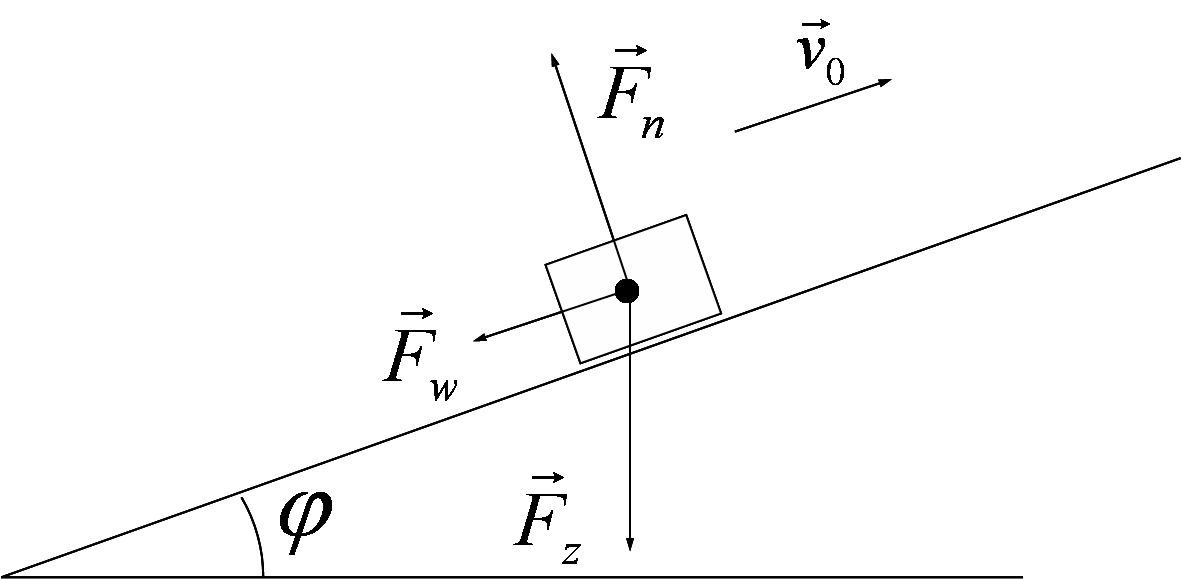
\includegraphics[width=0.49\textwidth,angle=0]{dyn/exercises/blok_helling_2}
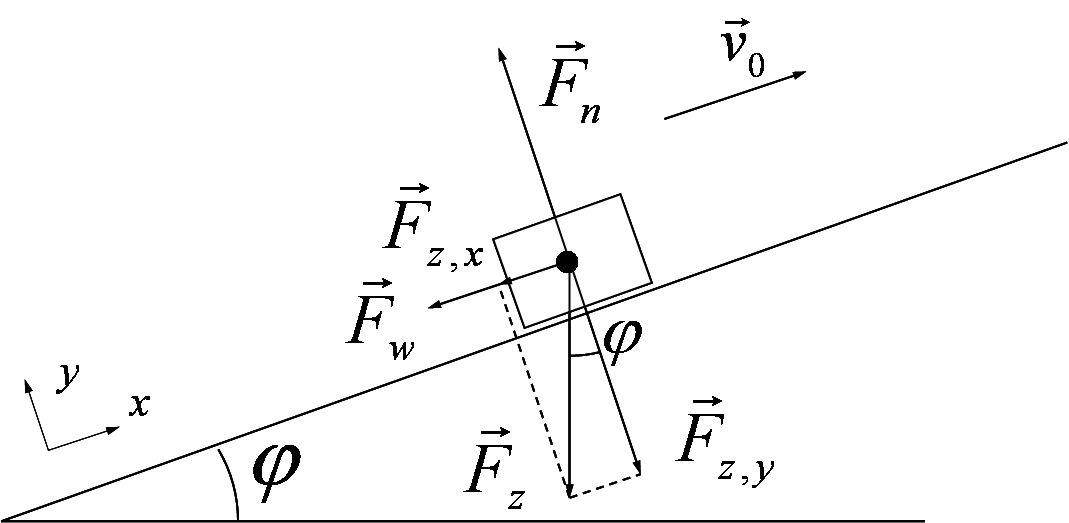
\includegraphics[width=0.49\textwidth, angle=0]{dyn/exercises/blok_helling_2componenten}
\end{flushright}
\end{figure}
$a=-\frac{F_w+mg\sin\varphi}{m}=-8,66\rm\,m/s^2$
\newline
$x=-\frac{v_0^2}{2a}=\frac{mv_0^2}{2(F_w+mg\sin\varphi)}=3,70\rm\,m$ %($t=0,92\rm\,s$) 
\newline
$F_{zx}>F_w$ zodat het blok terug naar beneden komt. 
\newline
$\mu=\frac{F_w}{mg\cos\varphi}=0,44$
\end{oplossing}



\end{exercise}

\begin{exercise} Een blok ligt op een helling. Bepaal de maximale hoek die de
helling kan maken met de horizontale zodat het blok n\'et niet in
beweging komt. De wrijvingsfactor is $\mu$.
\begin{oplossing}
\newline
We kiezen een assenstelsel met de $x$-as volgens de helling. De
zwaartekracht moeten we dan ontbinden in haar componenten.
\begin{eqnarray*}
\tan{\varphi}&=&\frac{F_{z,x}}{F_{z,y}}\\
&\Updownarrow&\\
F_{z,x}&=&F_{z,y}\tan{\varphi}\\
&=&F_n\tan{\varphi}\\
\end{eqnarray*}
Het blok is in rust zodat de $x$-component gelijk moet zijn aan de
wrij\-vings\-kracht. Omdat het blok nog net niet in beweging komt,
kunnen we de wrijvingskracht gelijkstellen aan $F_w=\mu F_n$. Dus:
\begin{eqnarray*}
F_w&=&F_n\tan{\varphi}\\
&\Downarrow&\\
\mu F_n&=&F_n\tan{\varphi}\\
&\Downarrow&\\
\mu&=&\tan{\varphi}
\end{eqnarray*}
De maximale hoek is ${\rm Bgtan\,}\mu$.
\end{oplossing}

\end{exercise}

\begin{exercise} Een steen wordt aan een touwtje in een horizontaal vlak rondgeslingerd met een snelheid die in grootte constant is. Heeft de steen een versnelling? Ondervindt de steen een resulterende kracht? Leg uit.


\end{exercise}

\begin{exercise} Een bestuurder van een auto met een massa van $1000~\rm kg$ rijdt aan een snelheid in grootte gelijk aan $10~\rm m/s$. Hij probeert een horizontale bocht, met een straal van $100~\rm m$ te nemen. De maximale wrijvingskracht tussen de banden en de baan is $900~\rm N$. Kan de auto deze bocht nemen of zal hij beginnen slippen?
\begin{oplossing}
\newline
\newline
De auto zal slippen in de bocht. Omdat we de snelheid en de straal kennen, kunnen we de versnelling van de gewenste cirkelbeweging berekenen. Met de tweede wet van Newton vinden we de (middelpuntzoekende) kracht nodig om deze versnelling te kunnen veroorzaken:
\begin{eqnarray*}
F&=&ma\\
&=&\frac{mv^2}{r}\\
&=&1000\rm\,N
\end{eqnarray*}
Dit is meer dan wat de grond maximaal op de wielen kan uitoefenen. De auto zal dus beginnen slippen.
\newline
\newline
Realiseer je dat de wrijvingskracht door de grond op de auto wordt uitgeoefend en de resulterende kracht vormt. Het is dan ook de middelpuntzoekende kracht. 
\begin{figure}[h]
\centering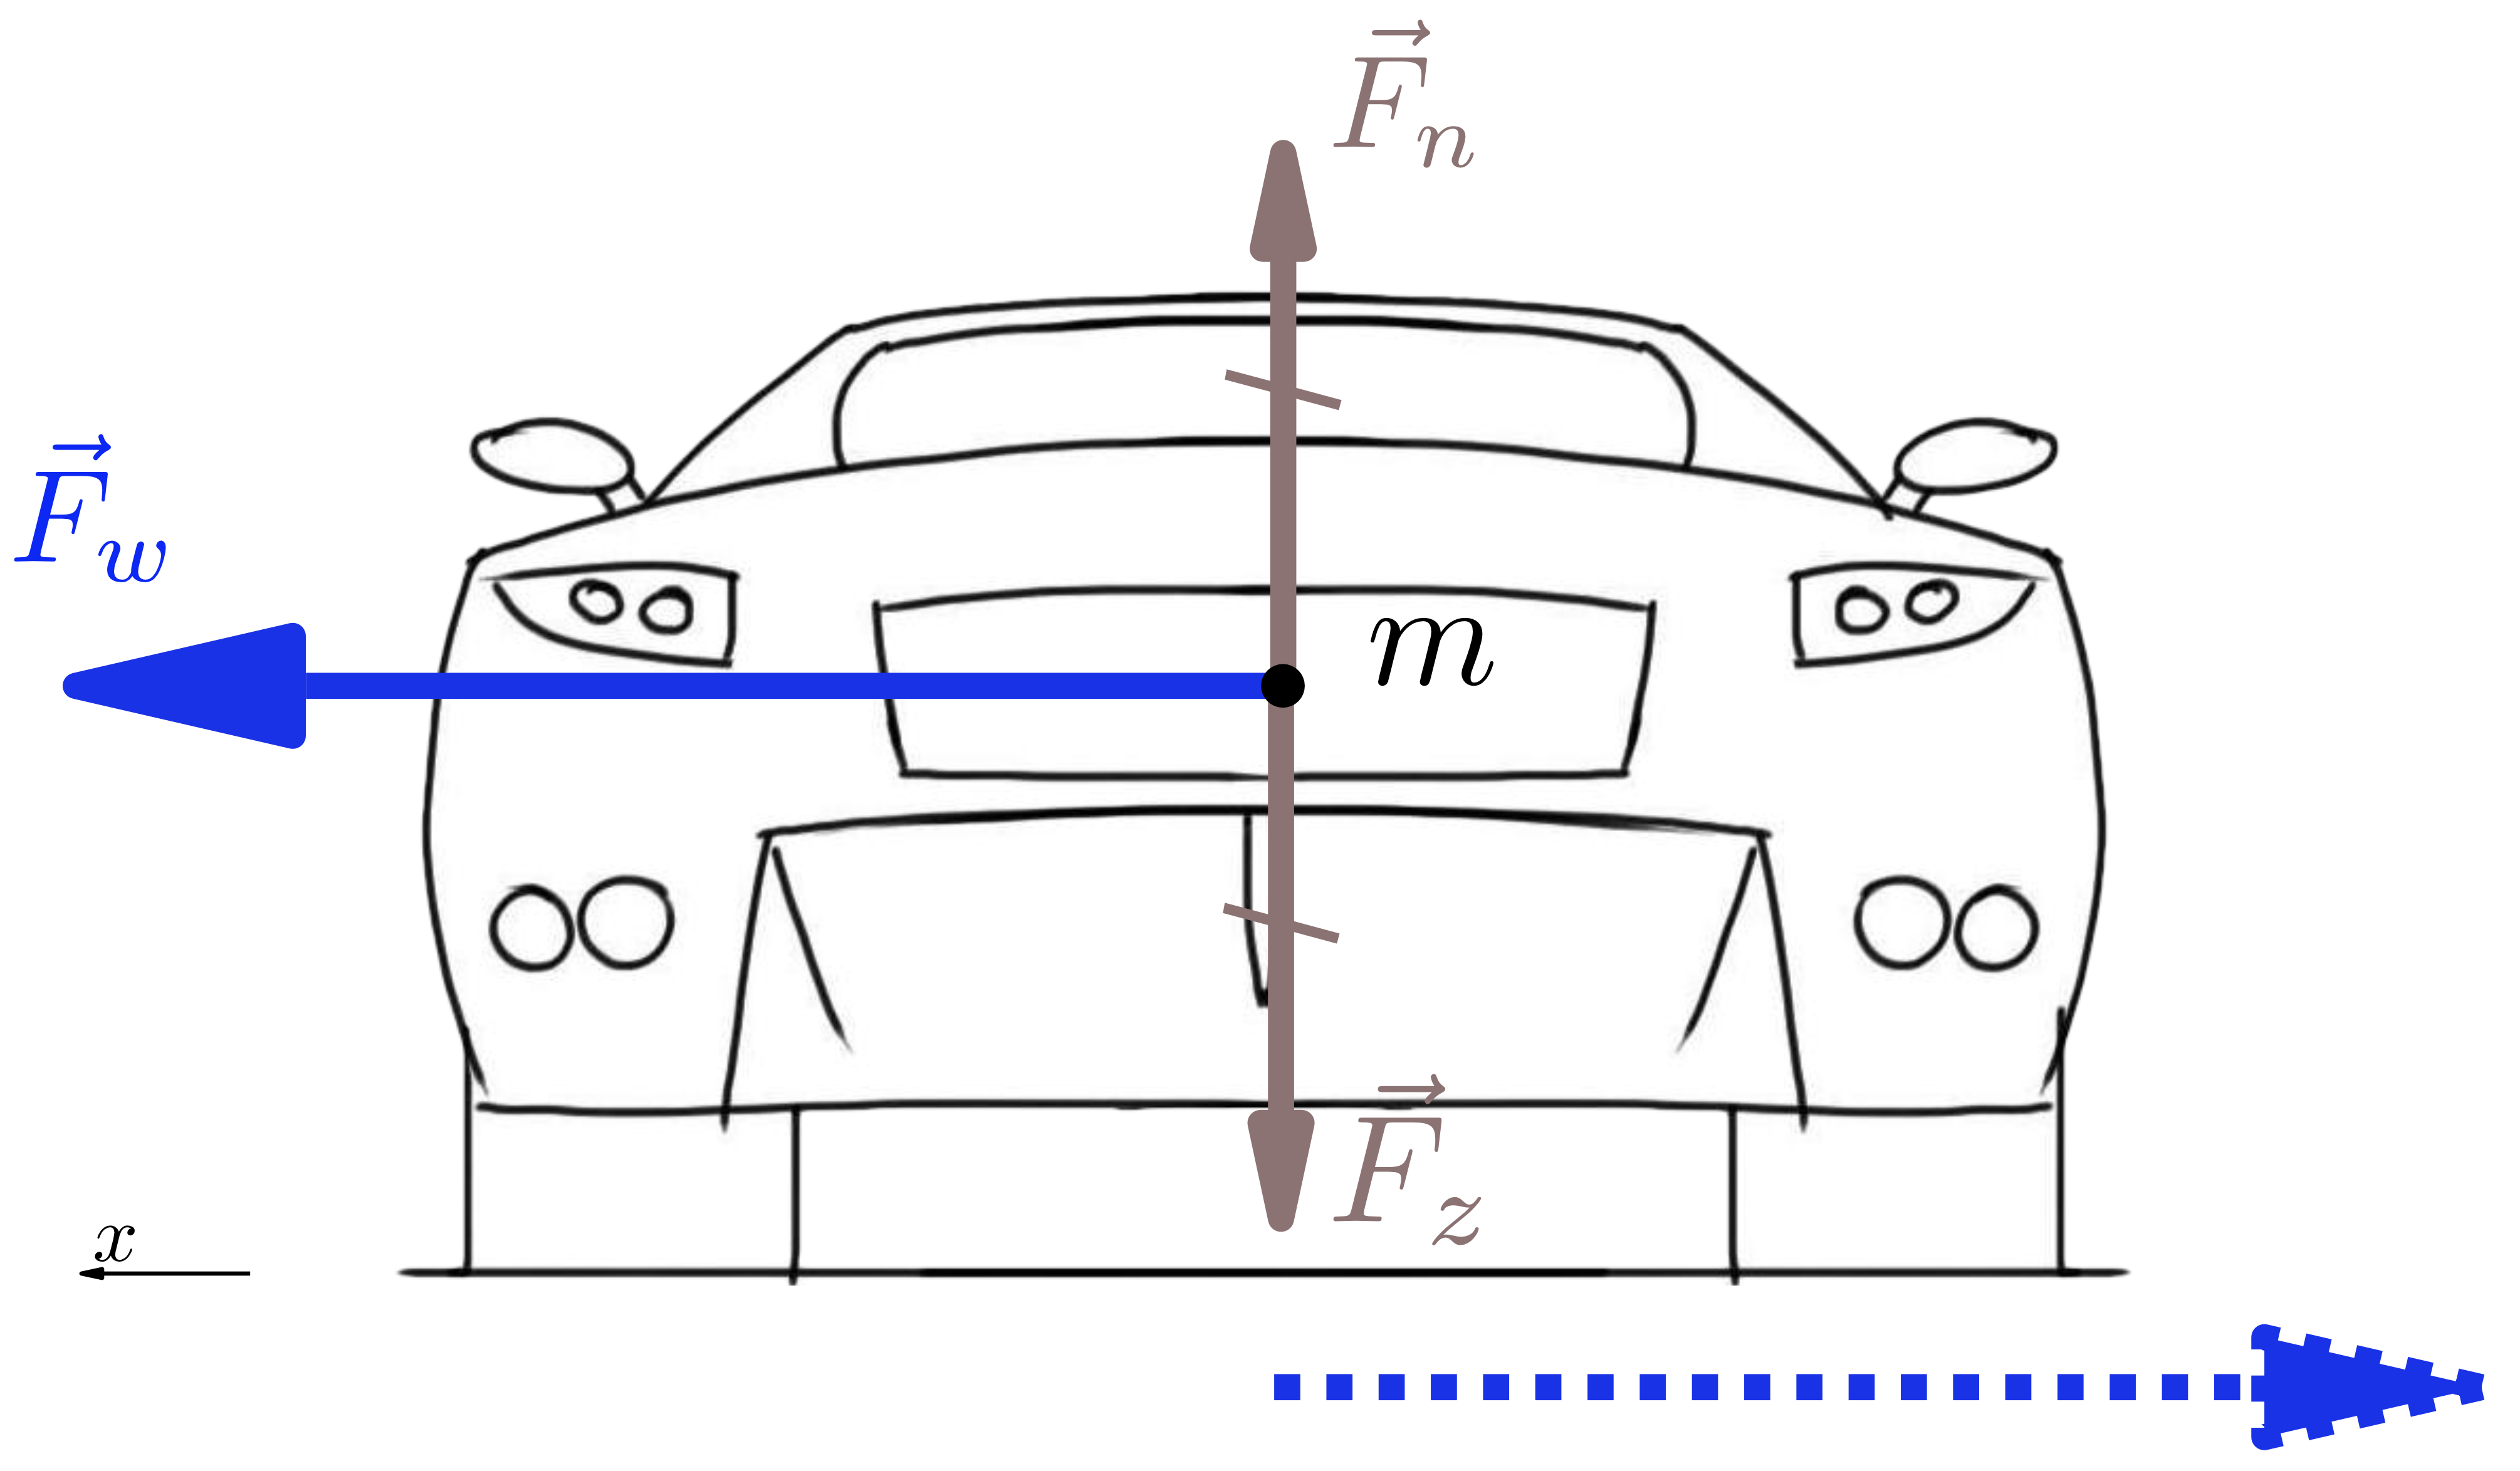
\includegraphics[width=0.5\textwidth, angle=0]{dyn/exercises/auto_bocht_horizontaal}
\end{figure}
De auto duwt met zijn wielen dwars ten opzichte van de snelheid tegen de grond en de grond duwt terug. In de figuur beweegt de auto het vlak van de tekening in en neemt de auto een bocht naar links (in de richting van de wrijvingskracht).
\end{oplossing}



\end{exercise}

\begin{exercise} Een cirkelvormige renbaan is onder een helling van $30^\circ$
gebouwd. De straal van de cirkel is $50~\rm m$. Met welke snelheid
moet een auto rijden om in de baan te blijven? Veronderstel dat de
baan spekglad is. 
\begin{oplossing}
\begin{figure}[h]
\centering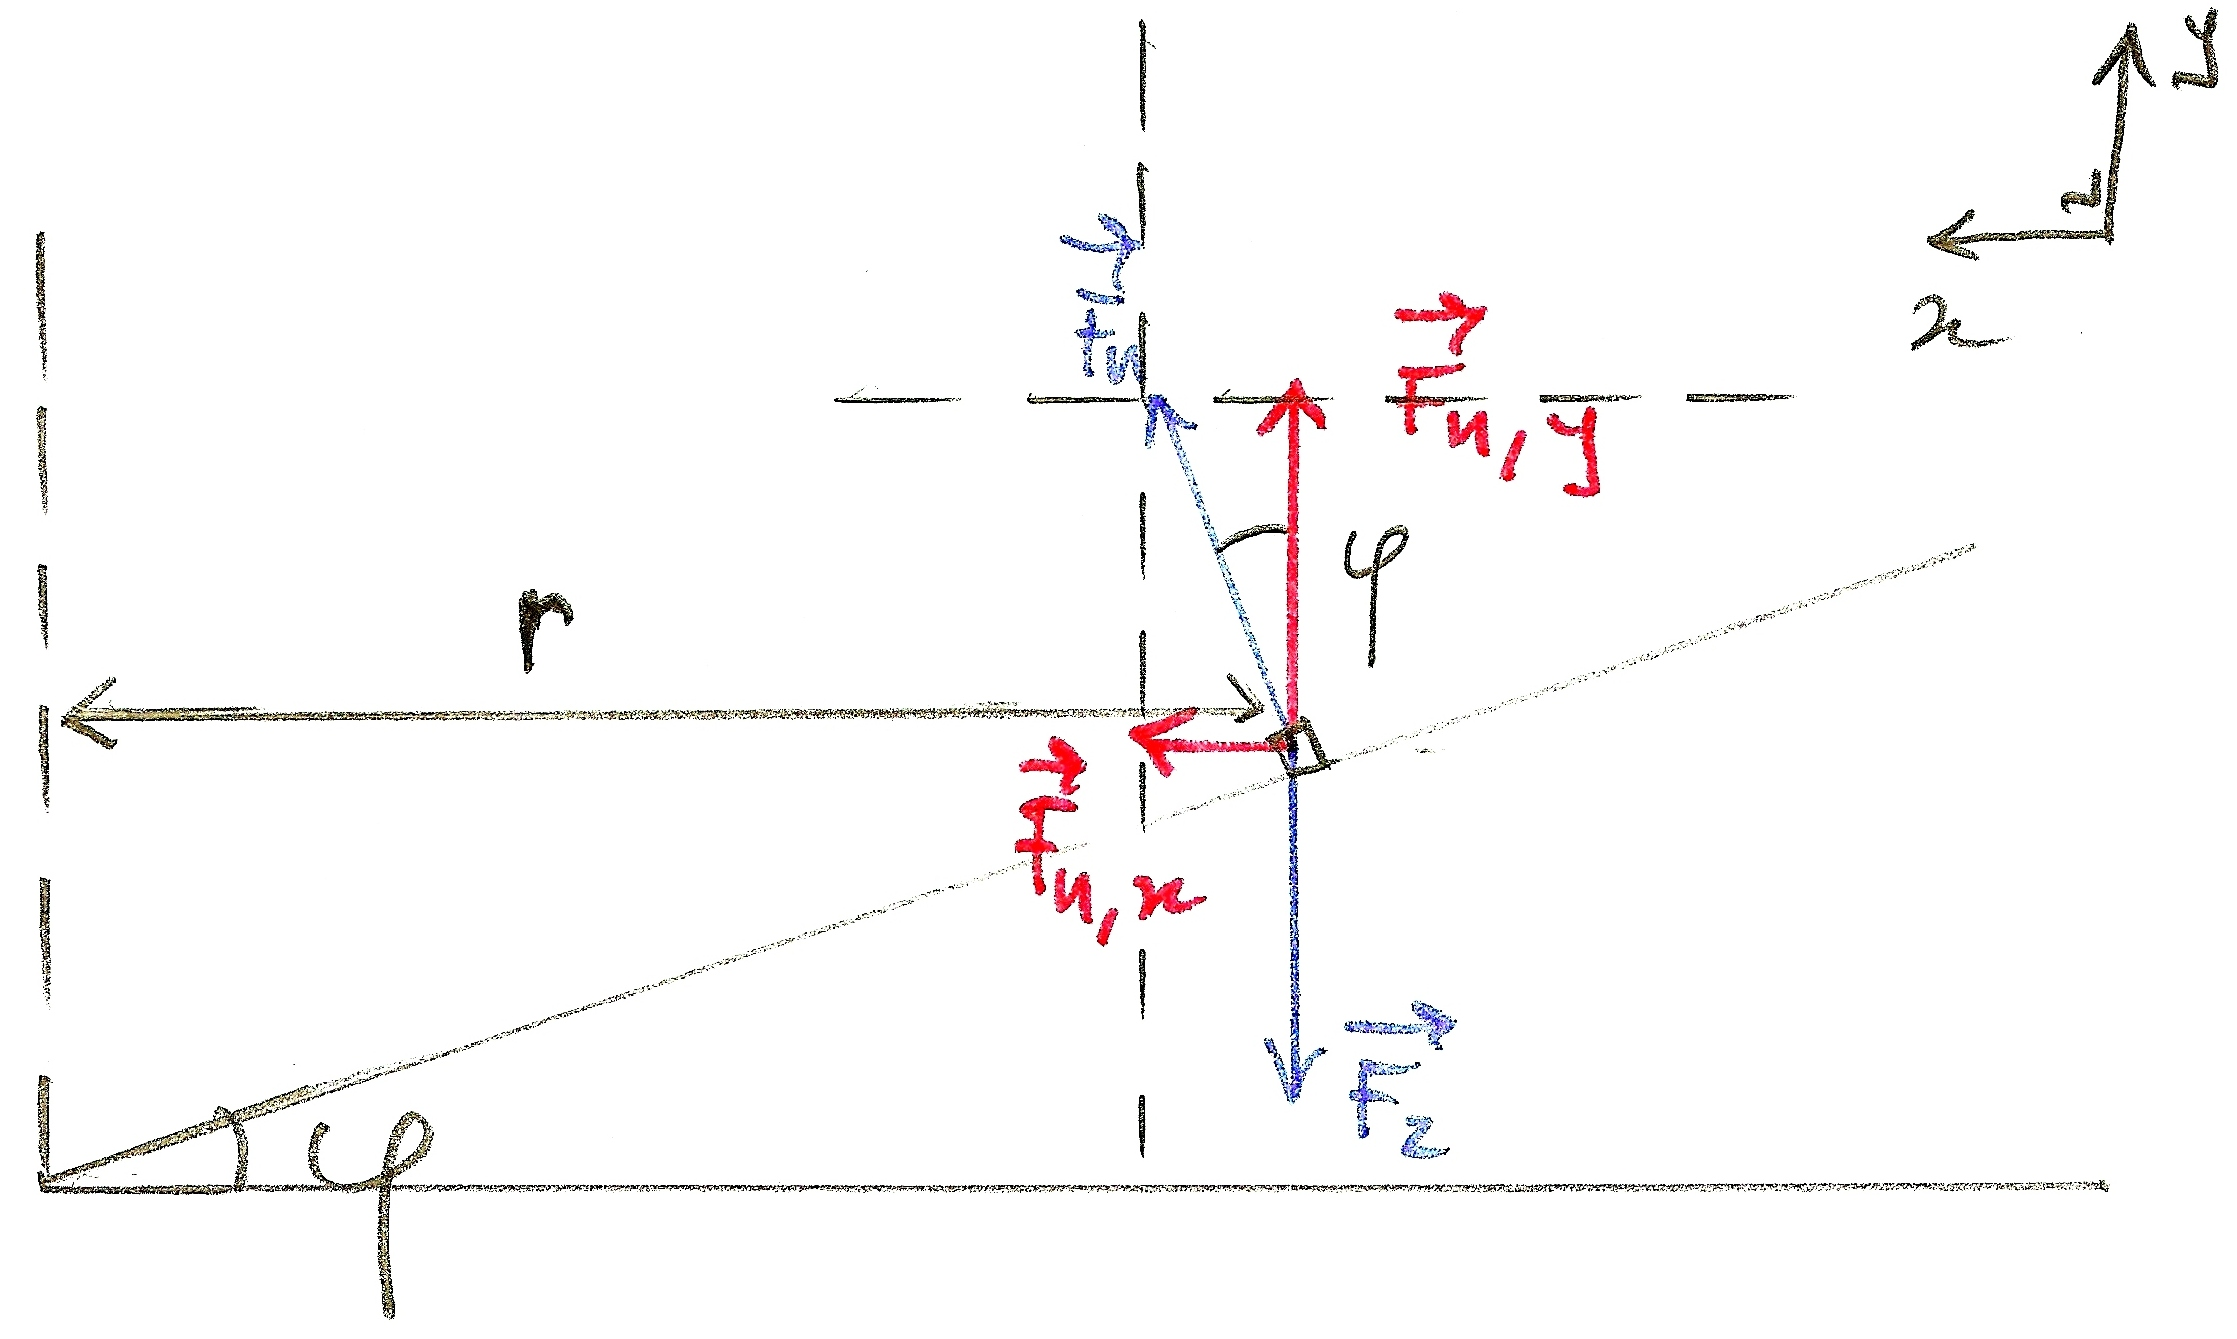
\includegraphics[width=0.6\textwidth, angle=0]{dyn/exercises/renbaan}
\end{figure}


\textit{gegeven}: $\varphi=30^\circ$\newline$r=50\rm\,m$

\textit{gevraagd:} $v$

\textit{oplossing:} De krachten die op de auto aangrijpen, zijn de zwaartekracht en de normaalkracht. In de $y$-richting is er geen versnelling omdat de auto in een horizontaal vlak beweegt. We kiezen dan ook een assenstelsel met de $y$-as verticaal geori\"enteerd. De $x$-as kunnen we in de richting van het centrum van de cirkel nemen. De $y$-component van de normaalkracht moet dus even groot zijn als de zwaartekracht. De $x$-component van de normaalkracht is dan ook de resulterende kracht en levert de middelpuntzoekende kracht. De $x$-component van de normaalkracht kunnen we m.b.v. de hoek en de zwaartekracht schrijven.
\newline
\newline
De $x$-component van de normaalkracht:
\begin{eqnarray*}
\tan{\varphi}&=&\frac{F_{n,x}}{F_{n,y}}\\
&\Updownarrow&\\
F_{n,x}&=&F_{n,y}\tan{\varphi}\\
&=&mg\tan{\varphi}
\end{eqnarray*}
We passen de tweede wet van Newton toe:
\begin{eqnarray*}
\vec{F}&=&m\vec{a}\\
&\Downarrow&\\
F_{n,x}&=&ma\\
mg\tan{\varphi}&=&\frac{mv^2}{r}\\
%&\Downarrow&\\
v&=&\sqrt{gr\tan{\varphi}}
\end{eqnarray*}
De gegevens invullen levert een snelheid van $17\rm\,m/s$.
\end{oplossing}

%\newpage


\end{exercise}

\begin{exercise} Op een draaitafel draait met een constante hoeksnelheid een grammofoonplaat. Twee muntstukken A en B zijn op zo'n plaats van het middelpunt van de draaitafel geplaatst dat zij nog net niet wegschuiven. Voor muntstuk A bedraagt de afstand tot de rotatieas dan $6\rm\,cm$ en voor B is het dan $12\rm\,cm$. $m_a$ en $m_b$ zijn de massa's van respectievelijk de muntstukken A en B. $\mu_a$ en $\mu_b$ zijn de wrijvingsfactoren tussen de muntstukken en de grammofoonplaat.
\newline
Welke gevolgtrekking m.b.t. de massa's en de wrijvingsfactoren is juist?
\newline
\newline
\begin{tabularx}{\textwidth}{*4{X}}
(a) $\displaystyle\mu_a=\frac{\mu_b}{2}$ & (b) $\displaystyle m_a=2m_b$ & (c) $\displaystyle m_a=\frac{m_b}{2}$ & (d)	$\displaystyle\frac{m_a}{\mu_a}=2\frac{m_b}{\mu_b}$
\end{tabularx}
\begin{oplossing}
Het juist antwoord is A. De wrijvingskracht tussen de muntjes en de
draaitafel moet voor de middelpuntzoekende kracht op de muntjes
zorgen. Als de muntjes nog n\'et niet wegschuiven, mogen we de
formule $F_w=\mu F_n$ voor de wrij\-vings\-kracht gebruiken. Dit
levert, met $F_n=F_z=mg$:
\begin{eqnarray*}
F&=&ma\\
&\Downarrow&\\
\mu mg&=&mr\omega^2\\
&\Downarrow&\\
\frac{\mu_a}{\mu_b}&=&\frac{r_a\omega^2}{g}\cdot\frac{g}{r_b\omega^2}\\
&=&\frac{r_a}{r_b}\\
&=&\frac{1}{2}
\end{eqnarray*}
\end{oplossing}

\end{exercise}

\begin{exercise} Een speelgoedwagentje beweegt in een horizontale cirkel met straal
$2l$ en heeft een tijd $T$ nodig om een volledige cirkel te
beschrijven. Dit kan omdat aan het wagentje een veer vastgemaakt is
.De lengte van de veer in niet uitgerekte toestand is $l$. Het
wagentje versnelt waarbij de straal van de beschreven cirkel gelijk
wordt aan $3l$.
\newline
De tijd die het wagentje nu nodig heeft om een volledige cirkel te
beschrijven is dan gelijk aan:
\begin{enumerate}
\item $T$
\item $\frac{3}{4}T$
\item $\sqrt{\frac{3}{4}}T$
\item $\sqrt{\frac{4}{3}}T$
\end{enumerate}
\begin{oplossing}
\textit{gegeven}
\begin{tabular}[t]{lcl}
$r$&=&$2l$\\
$r'$&=&$3l$\\
\end{tabular}

\textit{gevraagd}
\begin{tabular}[t]{ll}
$T'/T$
\end{tabular}

\textit{oplossing} De veerkracht zorgt voor de middelpuntzoekende kracht. We leiden hieruit een uitdrukking af voor de periode:
\begin{eqnarray*}
F&=&ma\\
&\Downarrow&\\
k\Delta l &=& mr\omega^2\\
&=&  mr\left(\frac{2\pi}{T}\right)^2\\
&\Updownarrow&\\
T^2&=&\frac{4\pi^2mr}{k\Delta l}
\end{eqnarray*}
De verhouding van het kwadraat van de periodes wordt dan:
\begin{eqnarray*}
\frac{T'^2}{T^2}&=&\frac{4\pi^2mr'}{k\Delta l'}\cdot\frac{k\Delta l}{4\pi^2mr}\\
&&\\
&=&\frac{3l(2l-l)}{(3l-l)2l}\\
&&\\
&=&\frac{3}{4}\\
&\Downarrow&\\
T'&=&\sqrt{\frac{3}{4}}\,T
\end{eqnarray*}
Het juiste antwoord is C.
\end{oplossing}





\end{exercise}

\begin{exercise} Waarom vliegt bij het afschieten van een kanonskogel, het kanon niet even ver achteruit als dat de kogel vooruit vliegt?


\end{exercise}

\begin{exercise} Moet een fietser, die op een horizontale weg eenparig rechtlijnig fietst, toch blijven trappen? Verklaar.

\end{exercise}

\begin{exercise} Een fietser met een massa van $60,2\rm\,kg$ rijdt op een rechte baan met een constante snelheid die $25,0\rm\,km/h$ bedraagt. Hoe groot is de inwerkende resulterende kracht? 
\begin{oplossing}
De resulterende kracht is 0. De eerste wet van Newton zegt dat een voorwerp maar een ERB kan uitvoeren indien de resulterende kracht erop nul is. Zou er een van nul verschillende kracht op de fietser inwerken dan krijgt hij een versnelling. Je moet blijven trappen om een kracht te genereren die even groot is als de wrijvingskracht.
\end{oplossing}

\end{exercise}

\begin{exercise} Kareltje is net vier jaar geworden en vindt dat hij groot genoeg is om mama te helpen wanneer zij hem naar school brengt met de fiets. Vanuit zijn kinderstoel achterop zal hij mama flink in de rug duwen. Wat ziet Kareltje over het hoofd? 

\end{exercise}

\begin{exercise} Geef aan of de volgende uitspraken waar of vals zijn. Licht je antwoord toe.
\begin{enumerate}
\item Als een lichaam niet versnelt dan kan er geen kracht op werken. 
\item Bij een parachutist is de zwaartekracht even groot als de weerstandskracht -- die hij ondervindt van de lucht -- wanneer hij met zijn parachute met een constante snelheid naar beneden daalt. 
%\item Wanneer je een kilo meel aan de evenaar koopt krijg je minder meel dan wanneer je een kilo meel op de noordpool zou kopen.
\end{enumerate}


\end{exercise}

\begin{exercise} Toon aan dat de remweg van een remmende auto omgekeerd
evenredig is met de wrijvingsfactor. Veronderstel dat de wielen
glijden over het wegdek.

\end{exercise}

\begin{exercise} Als we de `effectieve zwaartekracht' in een centrifuge willen vergroten, wat is dan beter: de straal verdubbelen of de hoeksnelheid verdubbelen?

\end{exercise}

\begin{exercise} Stel dat we een emmer met water aan een touw rondslingeren in een verticaal vlak zodanig dat het water niet uit de emmer valt. Neemt het (schijnbaar) gewicht van het water in de emmer toe wanneer we de emmer met een grotere snelheid laten ronddraaien? Leg uit.

\end{exercise}

\begin{exercise} Er wordt wel gezegd dat in een wasmachine water uit het wasgoed wordt verwijderd doordat de centrifugaalkracht het water naar buiten trekt. Is dit correct? Leg uit.

\end{exercise}

\begin{exercise} Verklaar hoe een fietser op een horizontaal wegdek een bocht kan nemen. Bepaal ook de maximale snelheid waarmee je door een bocht met straal $r$ kan gaan, als de wrijvingsfactor tussen de weg en de banden $\mu$ is.

\end{exercise}

\begin{exercise} Geef de formule voor de grootte van de middelpuntzoekende kracht.

\end{exercise}

\begin{exercise} Welk punt heeft de grootste versnelling: een punt op de buitenrand
van een ronddraaiende cd, of een punt op de helft van de straal van
een cd die met een tweemaal zo grote hoeksnelheid ronddraait? Toon
je antwoord aan.

\end{exercise}





\subsection{Vraagstukken}


\begin{exercise} Om een ongeval te vermijden, drukt een bestuurder van een auto zijn remmen volledig in. Na een remspoor van \SI{90}{m} komt hij tot stilstand. De wrijvingsfactor tussen de wielen en de weg is gelijk aan \SI{0,500}{}. Bepaal de snelheid die hij voor het remmen had.

\begin{oplossing}
$v_0=\sqrt{2\mu gx}=\SI{29,71}{m/s}=\SI{107}{km/h}$
\end{oplossing}

\end{exercise}

\begin{exercise} Een massa van $50,0~\rm g$ wordt door een horizontale kracht van $0,065~\rm N$ voortbewogen. Hij legt
onder de werking van deze kracht en de wrij\-vings\-kracht vanuit de rusttoestand in $10,0~\rm s$ op een rechte baan een afstand af van $40,7~\rm m$. Hoe groot zijn de wrijvingskracht en de wrijvingsfactor?
\begin{oplossing}
\textit{gegeven}
\begin{tabular}[t]{lcl}
$m$ &$=$& $50,0\cdot10^{-3}~\rm kg$\\
$F$ &$=$& $0,065~\rm N$\\
$t$ &$=$& $10,0~\rm s$\\
$x$ &$=$& $40,7~\rm m$\\
\end{tabular}

\textit{gevraagd}
$F_w$, $\mu$

\textit{oplossing}
Uit de vergelijkingen voor een EVRB vinden we de versnelling:
\begin{eqnarray}
x &=& x_0+v_0t+\frac{1}{2}at^2\nonumber\\
&\Downarrow& \nonumber\\
a &=&\frac{2x}{t^2}\label{versn_a}
\end{eqnarray}
Volgens de $x$-as samen met (\ref{versn_a}) geldt:
\begin{eqnarray}
F-F_w&=&ma\nonumber\\
&\Downarrow& \nonumber\\
F_w &=& F-m\frac{2x}{t^2}\label{F_w}\\
&=& 65\cdot10^{-3}~{\rm N}-50,0\cdot10^{-3}~{\rm kg}\frac{2\cdot40,7~{\rm m}}{{10,0~{\rm s}}^2}\nonumber\\
&=& 0,024~\rm N\nonumber
\end{eqnarray}
Uit vergelijking (\ref{F_w}) en $F_w=\mu F_n=\mu mg$ volgt:
\begin{eqnarray*}
\mu &=& \frac{F}{mg}-\frac{2x}{gt^2}\\
&=& 0,050
\end{eqnarray*}
\end{oplossing}

\end{exercise}

\begin{exercise} Toon aan dat de remweg van een remmende auto omgekeerd
evenredig is met de wrijvingsfactor. Veronderstel dat de wielen
glijden over het wegdek.
%Zie oplossing opdracht 33 HB p. 111, hier vonden we (\ref{remvgl}):
\begin{oplossing}
\begin{eqnarray*}
\mu&=&\frac{v_0^2}{2gx}\\
&\Updownarrow&\\
x&=&\frac{v_0^2}{2g\mu}
\end{eqnarray*}
De remweg $x$ is dus omgekeerd evenredig met de wrijvingsfactor $\mu$.
\end{oplossing}

\end{exercise}

\begin{exercise} Een auto rijdt op een horizontale baan met een snelheid van
$108\rm\,km/h$. Als hij plots moet remmen, wat is dan zijn kleinste
remafstand in de veronderstelling dat de wielen schuiven over het
wegdek en de wrijvingsfactor tussen de wielen en de weg gelijk is
aan $0,500$?
%Zie oplossing opdracht 33 HB p. 111, hier vonden we (\ref{remvgl}):
\begin{oplossing}
\begin{eqnarray*}
\mu&=&\frac{v_0^2}{2gx}\\
&\Updownarrow&\\
x&=&\frac{v_0^2}{2g\mu}\\
&=&\frac{(30\rm\,m/s)^2}{2\cdot9,81\rm\,m/s^2\cdot0,500}\\
&=&91,7\rm\,m
\end{eqnarray*}
\end{oplossing}


\end{exercise}

\begin{exercise} Een massa van $10,0~\rm kg$ is aan touwen opgehangen zoals in de figuur. De hoek is $\theta=60^\circ$. Bepaal de spankrachten $F_1,~F_2$ en $F_3$ in het touw.
\begin{figure}[h]
\begin{center}
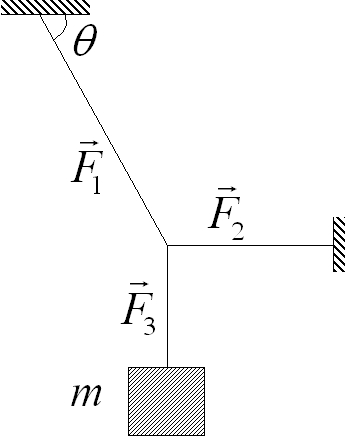
\includegraphics[width=.4\textwidth]{dyn/exercises/massa_aan_touw}
\end{center}
\end{figure}




\end{exercise}

\begin{exercise} Een zak cement met massa $m$ hangt aan drie touwen zoals weergegeven op de figuur. Twee van de drie touwen maken een hoek $\theta_1$, respectievelijk $\theta_2$ met de horizontale. Het geheel is in rust.
\begin{enumerate}
\item Bewijs dat de grootte van de spankracht in het linkertouw te berekenen is uit:
\[
F_1=\frac{mg\cos{\theta_2}}{\sin{(\theta_1+\theta_2)}}
\]
\item Als de massa van de cement $20,4\rm\,kg$ bedraagt, $\theta_1=10,0^\circ$ en $\theta_2=25,0^\circ$ hoe groot zijn dan de spankrachten in de drie touwen?
\end{enumerate}
\begin{oplossing}
\begin{enumerate}
\item In de horizontale $x$-richting is er geen versnelling zodat volgens de tweede wet van Newton de componenten van de krachten in deze rich\-ting elkaar moeten opheffen:
\begin{eqnarray}
\sum_{i=1}^3F_{i,x}&=&ma_x\nonumber\\
&\Updownarrow&\nonumber\\
F_{1,x}+F_{2,x}+F_{3,x}&=&ma_x\nonumber\\
&\Downarrow&\nonumber\\
-F_1\cos{\theta_1}+F_2\cos{\theta_2}+0&=&0\label{cement1}
\end{eqnarray}
Ook in de verticale $y$-richting moeten de krachten elkaar opheffen,
ook hier is er geen versnelling:
\begin{eqnarray}
F_1\sin{\theta_1}+F_2\sin{\theta_2}-mg&=&0\label{cement2}
\end{eqnarray}
We hebben twee vergelijkingen met twee onbekende krachten. We lossen
op naar $F_1$:
\begin{eqnarray}
(\ref{cement1})&\Leftrightarrow&F_2=\frac{F_1\cos{\theta_1}}{\cos{\theta_2}}\label{cement3}\\
(\ref{cement2})&\Leftrightarrow&F_2=\frac{mg-F_1\sin{\theta_1}}{\sin{\theta_2}}\nonumber
\end{eqnarray}
Deze uitdrukkingen aan elkaar gelijk stellen levert:
\begin{eqnarray*}
F_1\cos{\theta_1}\sin{\theta_2}&=&mg\cos{\theta_2}-F_1\sin{\theta_1}\cos{\theta_2}\\
&\Updownarrow&\\
F_1(\sin{\theta_1}\cos{\theta_2}+\cos{\theta_1}\sin{\theta_2})&=&mg\cos{\theta_2}\\
&\Updownarrow&\\
F_1&=&\frac{mg\cos{\theta_2}}{\sin{(\theta_1+\theta_2)}}
\end{eqnarray*}
\item Deze formule invullen in (\ref{cement3}) levert:
\begin{eqnarray*}
F_2&=&\frac{mg\cos{\theta_1}}{\sin{(\theta_1+\theta_2)}}
\end{eqnarray*}
\end{enumerate}
\end{oplossing}


\end{exercise}

\begin{exercise} Bereken de versnelling van het systeem in de figuur. De dynamische wrijvingsfactor is $\mu$ en het touw heeft een verwaarloosbare massa zodat de spankracht in het touw overal hetzelfde is. 
%figuur = blokken_op_helling.bmp


\end{exercise}

\begin{exercise} Drie voorwerpen zijn aan elkaar verbonden met touwtjes. De wrij\-vings\-factor tussen de tafel en het erop liggend voorwerp $V$ is $\mu$.
\begin{figure}[h]
\begin{center}
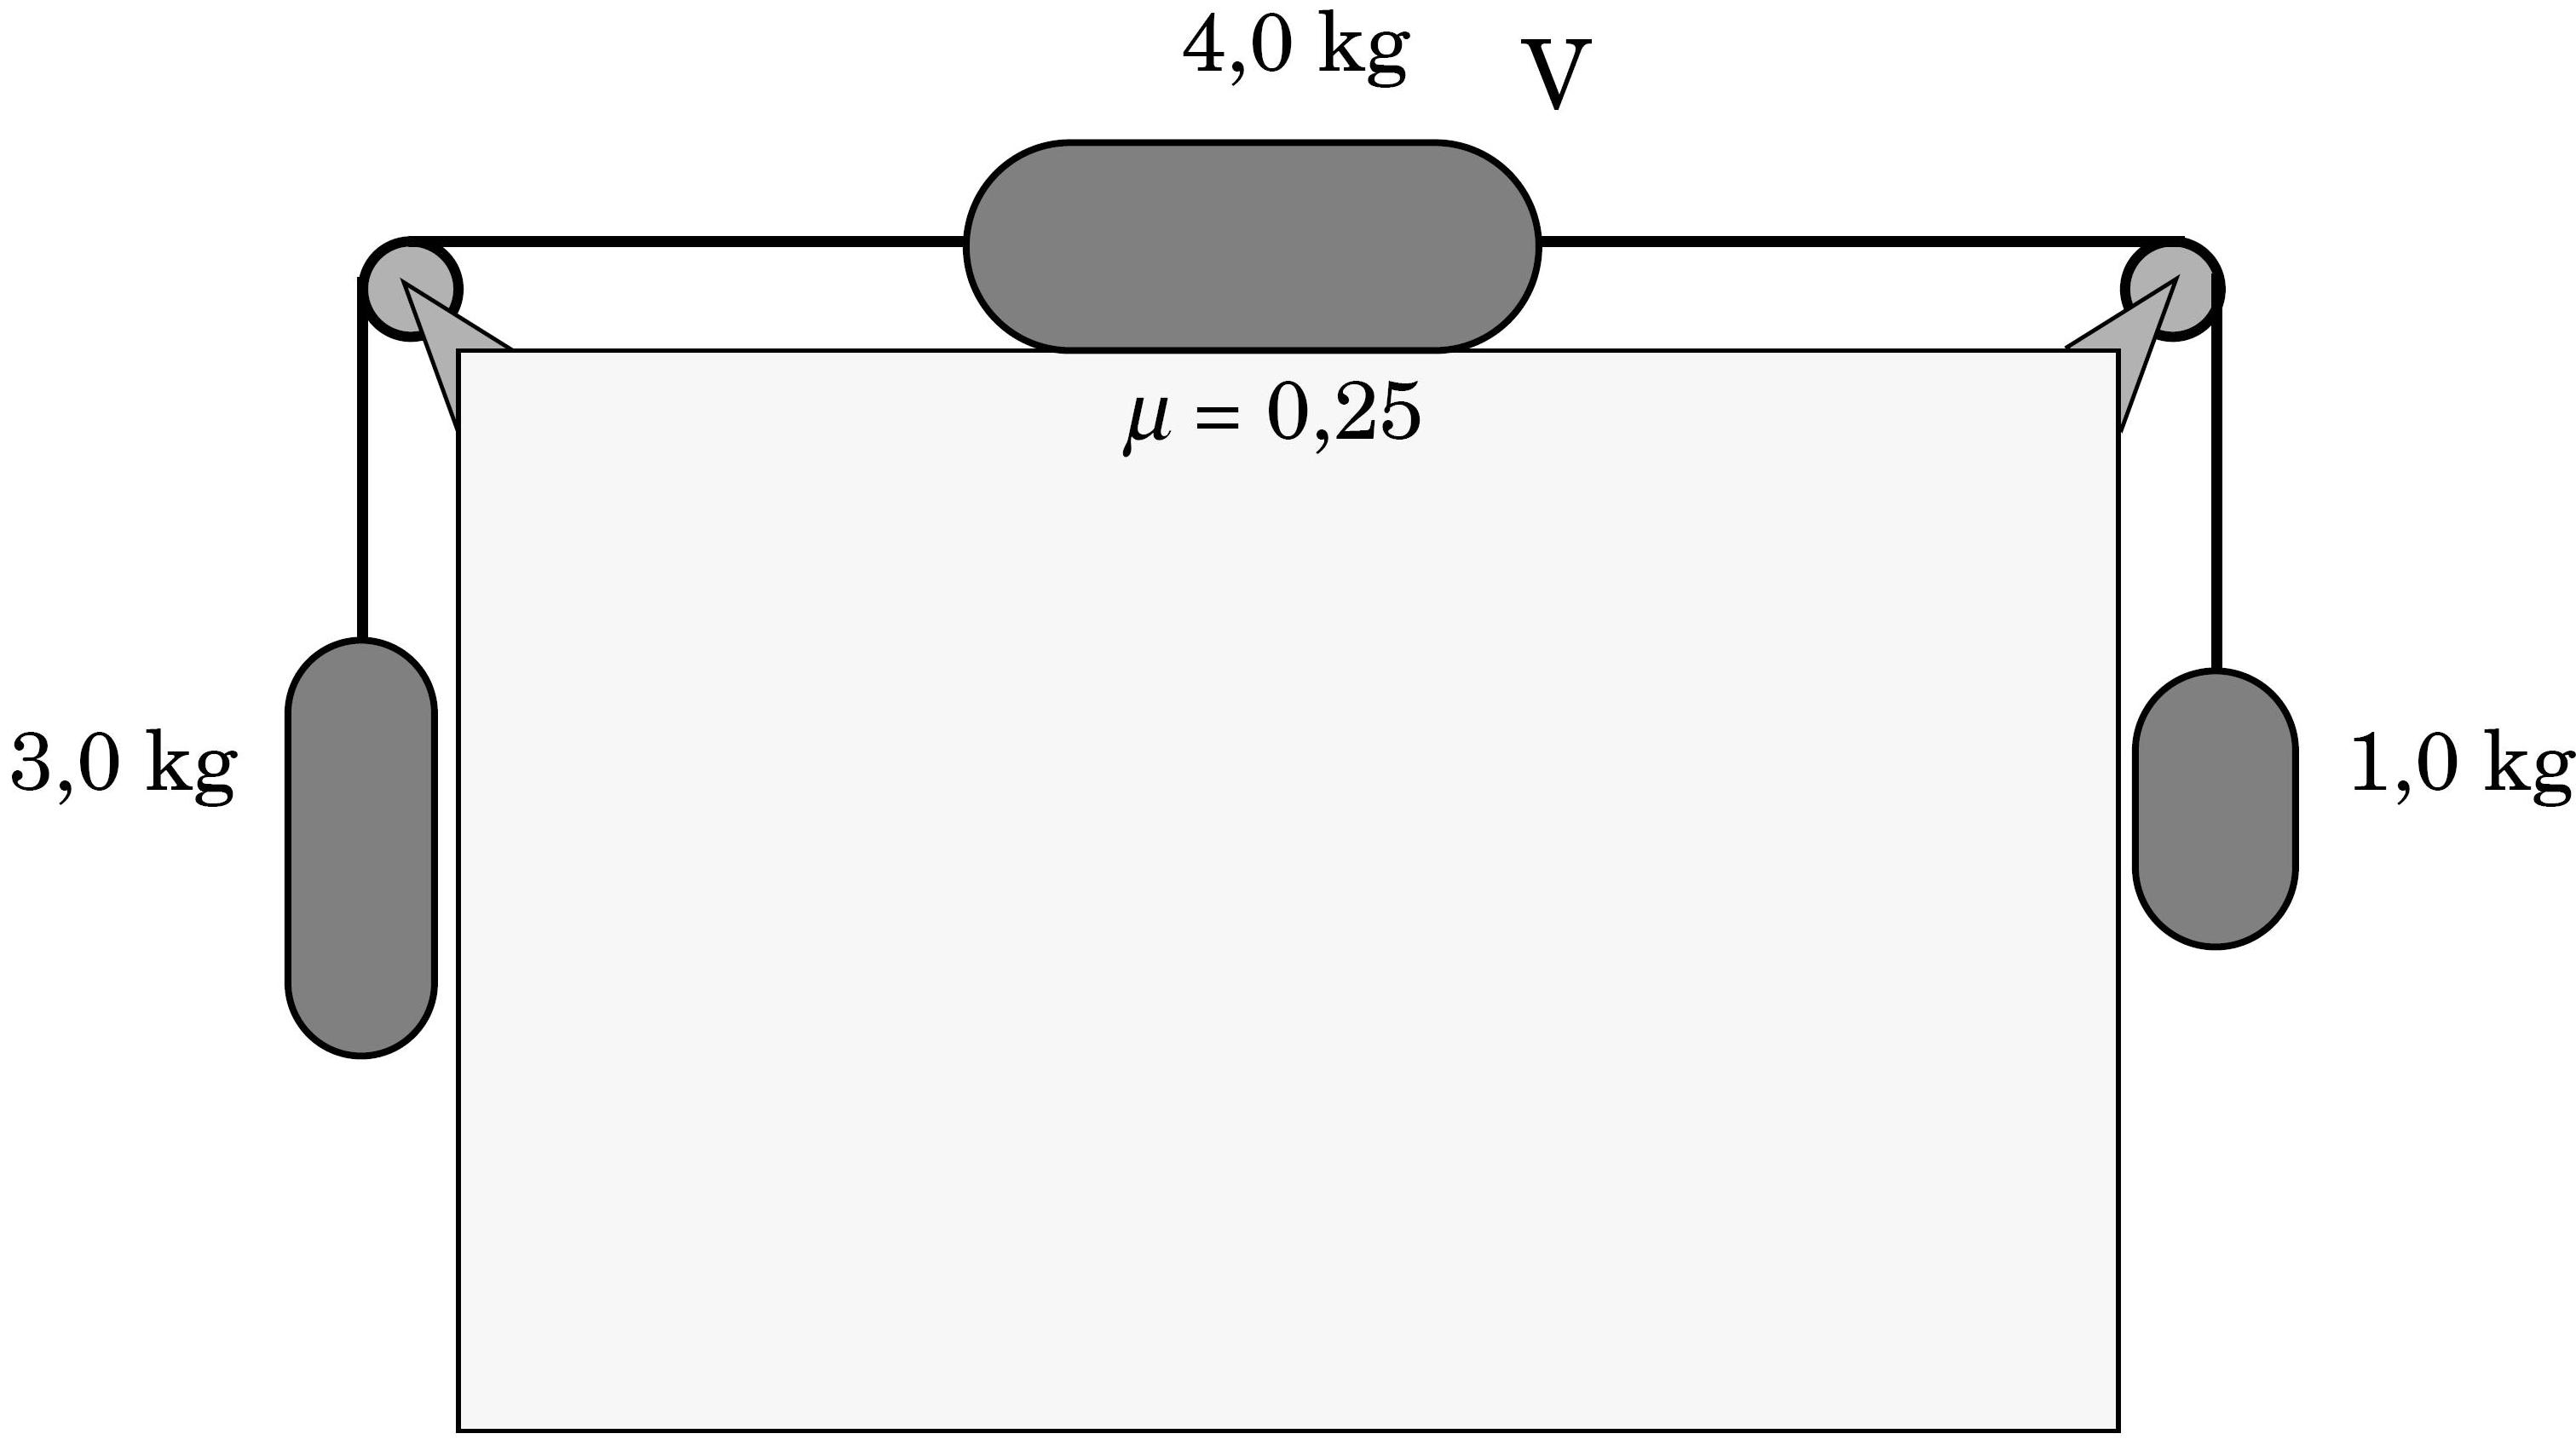
\includegraphics[width=0.6\textwidth ,angle=0]{dyn/exercises/drie_voorwerpen}
\end{center}
\end{figure}
Veronderstel dat er geen wrijving is in de katrollen en dat de massa van de katrollen te verwaarlozen is. Bepaal de versnelling van het voorwerp. \footnote{Bron: 16de VFO 2004}
\begin{oplossing}
\newline
Om de versnelling van het voorwerp te vinden kunnen we de tweede wet van Newton toepassen op de drie massa's. We tekenen de krachtendiagrammen op elk van de massa's (zie figuur). 
\begin{figure}[h]
\begin{center}
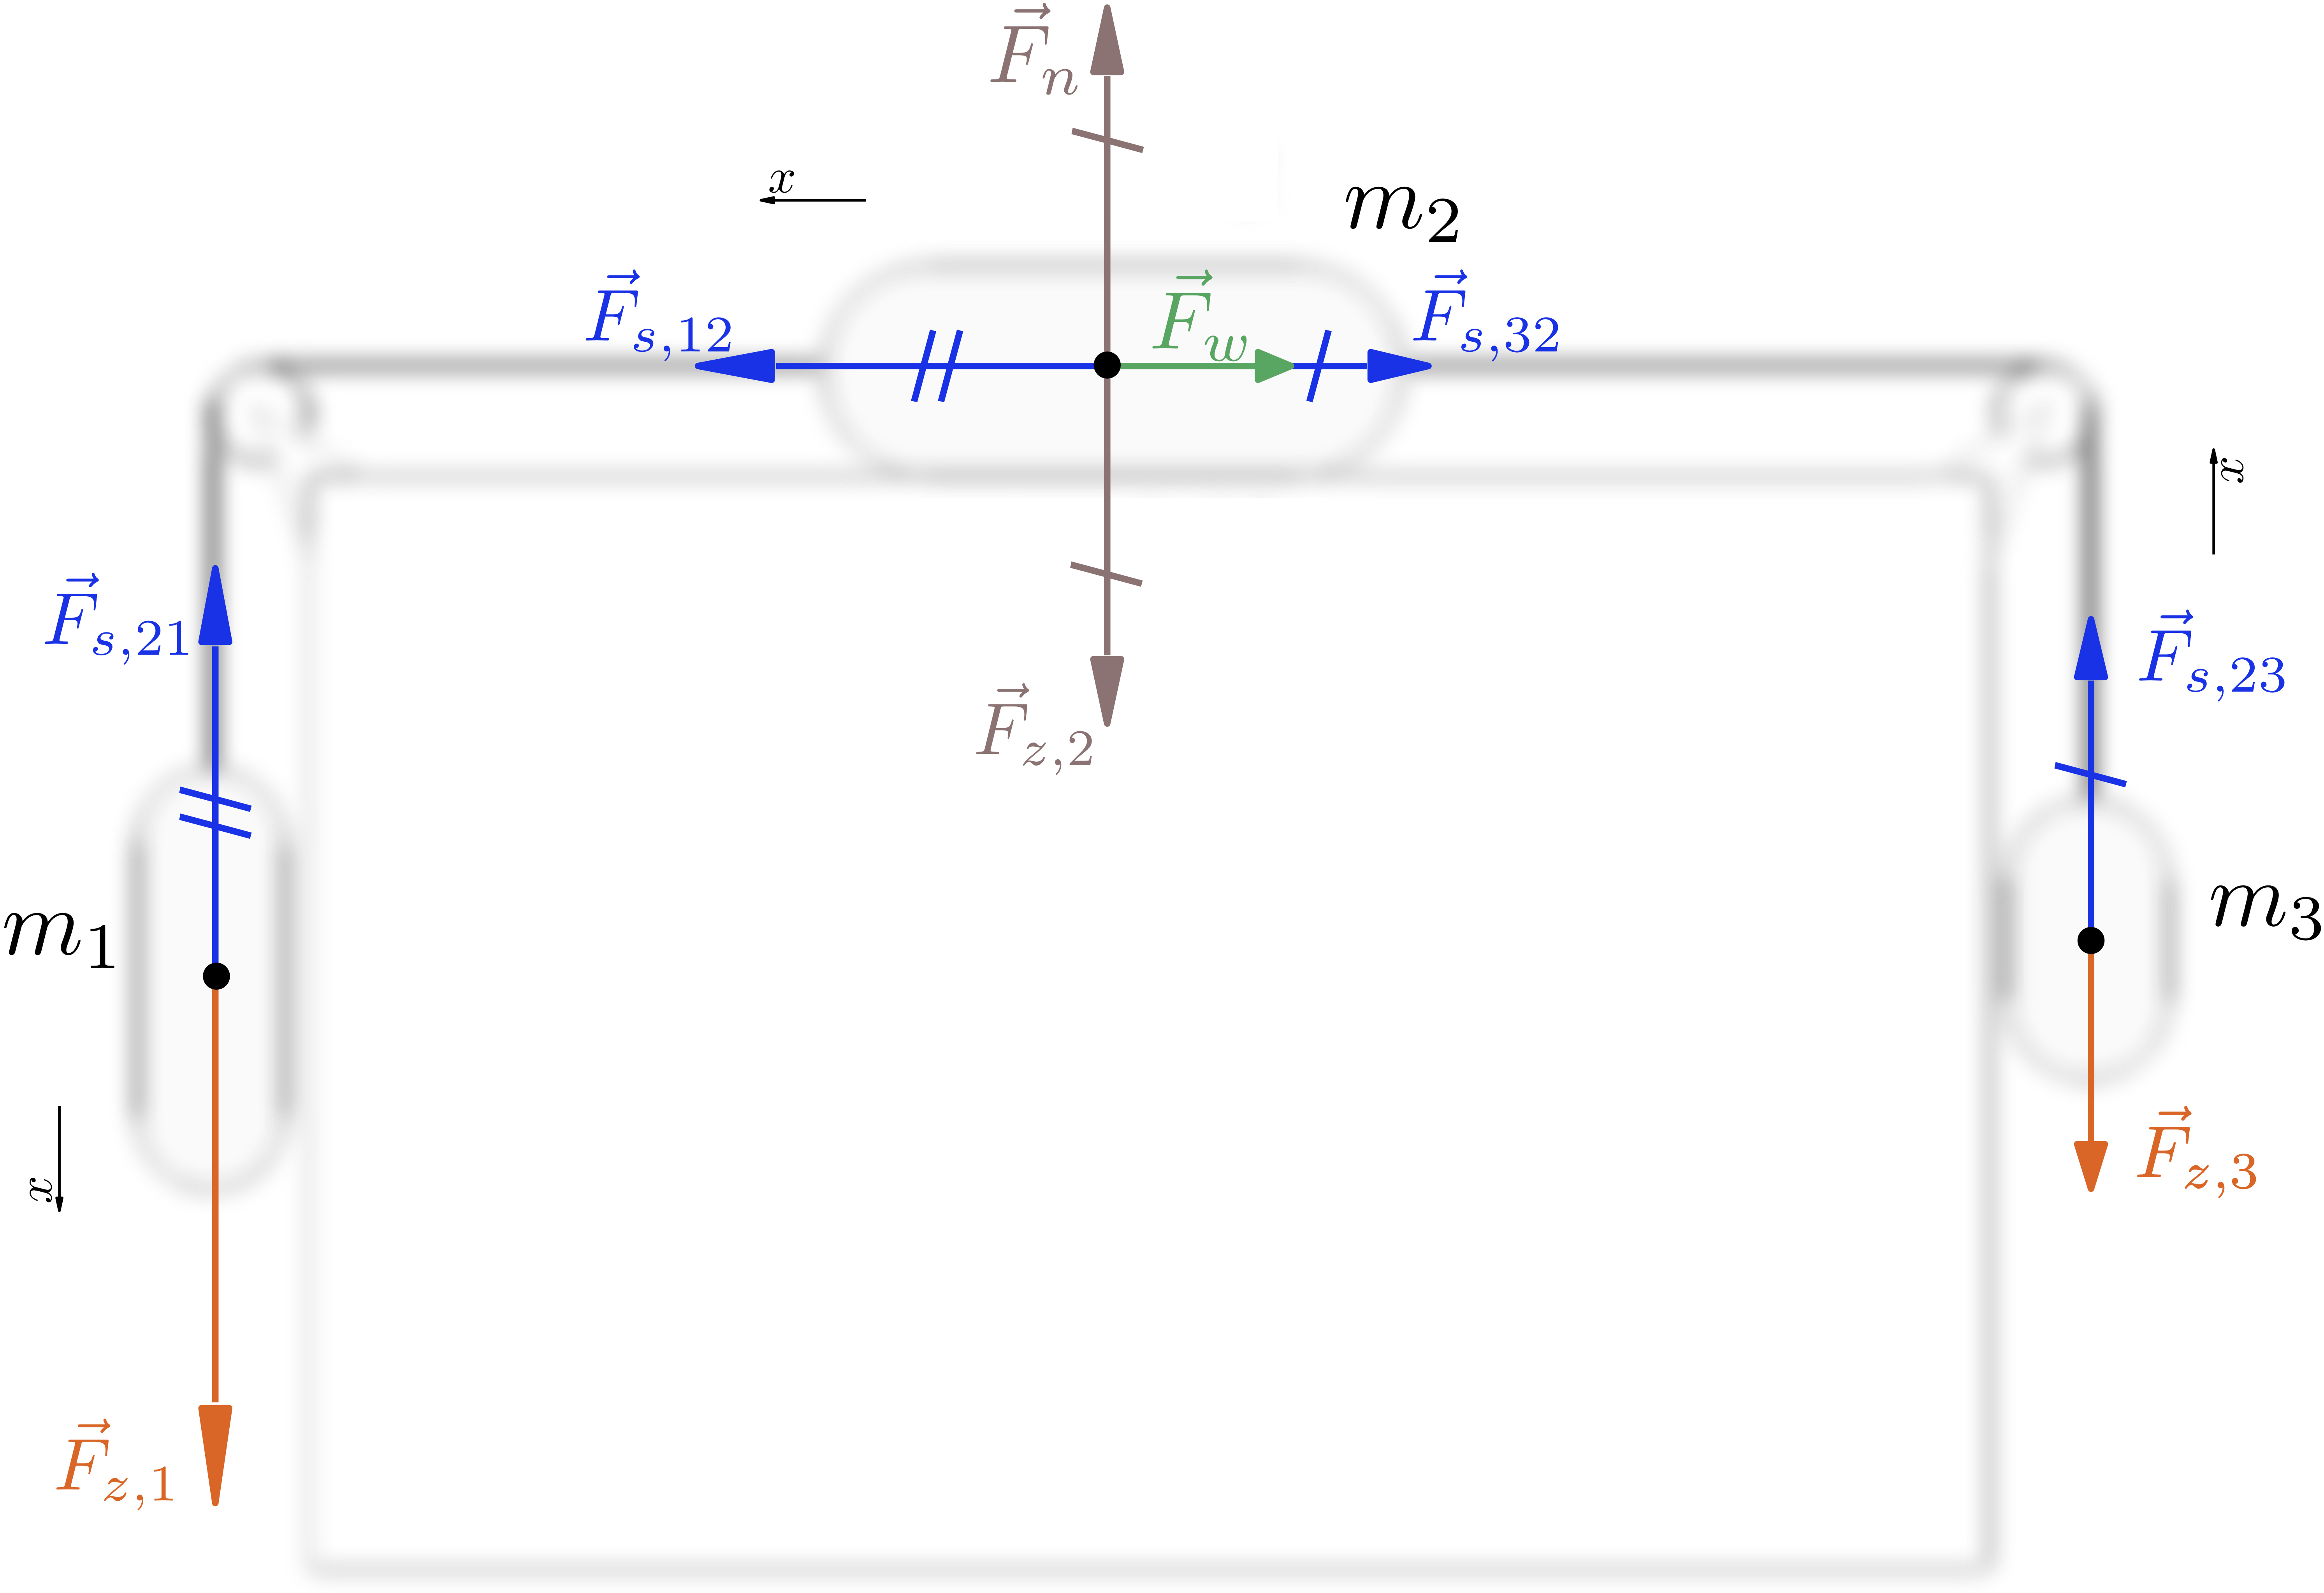
\includegraphics[width=0.73\textwidth ,angle=0]{dyn/exercises/drie_voorwerpen_krachten}
\end{center}
\end{figure}
\newline
Voor $m_1$ vinden we, met de keuze van de $x$-as verticaal naar beneden:
\begin{eqnarray}
F_{z,1}-F_{s,21}=m_1a\label{m_1}
\end{eqnarray}
Voor $m_3$ vinden we, met nu de keuze van de $x$-as verticaal naar boven:
\begin{eqnarray}
F_{s,23}-F_{z,3}=m_3a\label{m_3}
\end{eqnarray}
Voor $m_2$ vinden we, met de keuze van de $x$-as horizontaal naar links:
\begin{eqnarray}
F_{s,12}-F_w-F_{s,32}=m_2a\label{m_2}
\end{eqnarray}
Volgens de derde wet van Newton kunnen we de overeenkomstige spankrachten aan mekaar gelijk stellen: $F_{s,21}=F_{s,12}$ en $F_{s,32}=F_{s,23}$. Samen met $F_w=\mu F_n$ en $F_z=ma$ hebben we drie vergelijkingen en drie onbekenden. Oplossen naar de versnelling levert:
\begin{eqnarray*}
a=\frac{m_1-m_2-\mu m_3}{m_1+m_2+m_3}g=1,226\rm\,m/s^2
\end{eqnarray*}
\newline
\newline
Realiseer je dat de keuze van de $x$-as bij het bepalen van de componenten van de krachten de tekens bepalen van die componenten -- en ook die van de versnelling. Als je bijvoorbeeld tweemaal $a$ schrijft (in vergelijking (\ref{m_1}) en (\ref{m_3})) moet het ook effectief over dezelfde versnelling gaan, en niet over versnellingen die elkaars tegengestelde zijn. Met de $x$-as verticaal naar beneden geori\"enteerd voor $m_1$, zal de versnelling voor $m_1$ positief zijn als de massa naar beneden versnelt (wat hij doet; $m_1>m_3$). Voor $m_3$ moet je dan de $x$-as verticaal omhoog kiezen, wil je dat $a$ evenzeer positief is of dus dezelfde betekenis heeft.
\newline
\newline
Zie ook dat uit vergelijking (\ref{m_1}) volgt dat $m_1$ niet met de zwaartekracht aan $m_2$ trekt! De massa $m_1$ versnelt, waarvoor een resulterende kracht nodig is. 
\end{oplossing}



\end{exercise}

\begin{exercise} Een last van 1000 N hangt aan een kabel van $5,00\rm\,m$
lengte. Deze last wordt door een horizontale kracht $2,00\rm\,m$
zijwaarts uit zijn verticale stand getrokken.
\begin{enumerate}
    \item Bepaal de kracht waarmee zijwaarts aan de last werd
    getrokken.
    \item Bepaal de kracht waaraan het touw minimaal moet kunnen
    weerstaan zonder te breken.
\end{enumerate}


\end{exercise}

\begin{exercise} Als een persoon in vrije val ten gevolge van de
wrijvingskracht met de lucht valt met een maximumsnelheid van
ongeveer $240\rm\,km/h$ en deze wrijvingskracht is recht evenredig
met het kwadraat van de snelheid, bepaal dan deze
evenredigheidsconstante (= de wrijvinfsco\"effici\"ent). De persoon
heeft een massa van $66\rm\,kg$.


\begin{oplossing}
    \begin{itemize}
\item[24 p.72]Misschien eerst ter verduidelijking: de aangeduide kracht kan bijvoorbeeld worden uitgeoefend door een gewicht dat aan punt $A$ is opgehangen. Om de gevraagde krachten te vinden, kunnen we de gegeven kracht ontbinden. We kunnen haar beschouwen als samengesteld uit twee krachten. Namelijk de kracht op de staaf uitgeoefend ($\vec{F}_{ab}$, de staaf ondersteunt punt $A$) en de kracht waarmee aan het touw wordt getrokken ($\vec{F}{ac}$, het touw voorkomt dat $A$ naar beneden zou vallen zodat m.a.w. het punt aan het touw moet trekken).
    \begin{figure}[h]
    \centering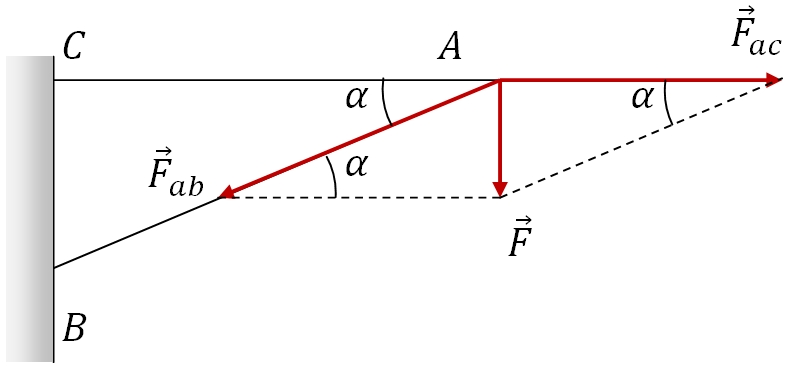
\includegraphics[width=0.7\textwidth]{dyn/exercises/24p72_fig}
    \end{figure}
    \newline
    Voor $F_{ab}$ geldt:
    \begin{eqnarray*}
    \sin{\alpha}&=&\frac{F}{F_{ab}}\\
    &\Updownarrow&\\
    F_{ab}&=&\frac{F}{\sin{\alpha}}=\frac{1500\rm\,N}{\frac{1}{2}}=3,00\cdot10^3\rm\,N
    \end{eqnarray*}
    Voor $F_{ac}$ geldt:
    \begin{eqnarray*}
    F_{ac}&=&\frac{F}{\tan{\alpha}}=\frac{1500\rm\,N}{\frac{\sqrt{3}}{3}}=2,60\cdot10^3\rm\,N
    \end{eqnarray*}

\item[25 p.72]De zwaartekracht werkt verticaal naar beneden, grijpt aan op de massa en wordt door de aarde uitgeoefend. Ook de spankracht werkt op de massa. Deze wordt door het touw op de massa uitgeoefend. Ze is altijd volgens het touw gericht. Naast de wrijvingskracht die we hier buiten beschouwing laten, zijn dit de enige twee krachten die op de slingerende massa werken.

\item[27 p.73]De versnelling die een voorwerp met massa $m$ krijgt als gevolg van een kracht $F$, is volgens de tweede wet van Newton gelijk aan $a=\frac{F}{m}$ zodat:
\begin{eqnarray*}
v=at=\frac{Ft}{m}=10\rm\,m/s
\end{eqnarray*}

\item[29 p.73]Uit de formules voor een EVRB kunnen we een uitdrukking voor de vertraging vinden (zie voor de uitwerking de oplossingen van vraagstukken die we maakten in de kinematica):
\[
a=-\frac{v_0^2}{2x}
\]
Om deze vertraging te kunnen realiseren is volgens de tweede wet van Newton een kracht nodig gelijk aan:
\begin{eqnarray*}
F=ma=-m\frac{v_0^2}{2x}=-37500\rm\,N
\end{eqnarray*}
Het minteken slaat op het feit dat de kracht tegengesteld is aan de snelheid die met de keuze van de $x$-as mee is. De grootte van de kracht is dan de uitdrukking zonder het minteken.
\end{itemize}
\end{oplossing}

\begin{oplossing}
    \begin{itemize}

\item [36 p.112]
Het juist antwoord is B. $v_{max}=\sqrt{\mu rg}$ dus $v_{max}\sim\sqrt{r}$.

\item [37 p.112]
$v_{max}\sim\sqrt{r}$ dus moeten we $v_{max}$ uitzetten tegen
$\sqrt{r}$.
    \end{itemize}
\end{oplossing}



\end{exercise}

\begin{exercise} Een blokje op een wrijvingsloze tafel beschrijft een ECB doordat het vastgemaakt is aan een koordje dat door een
gaatje in de tafel gaat en waaraan een massa is verbonden die door
de zwaartekracht naar beneden wordt getrokken.
\begin{figure}[h]
\begin{center}
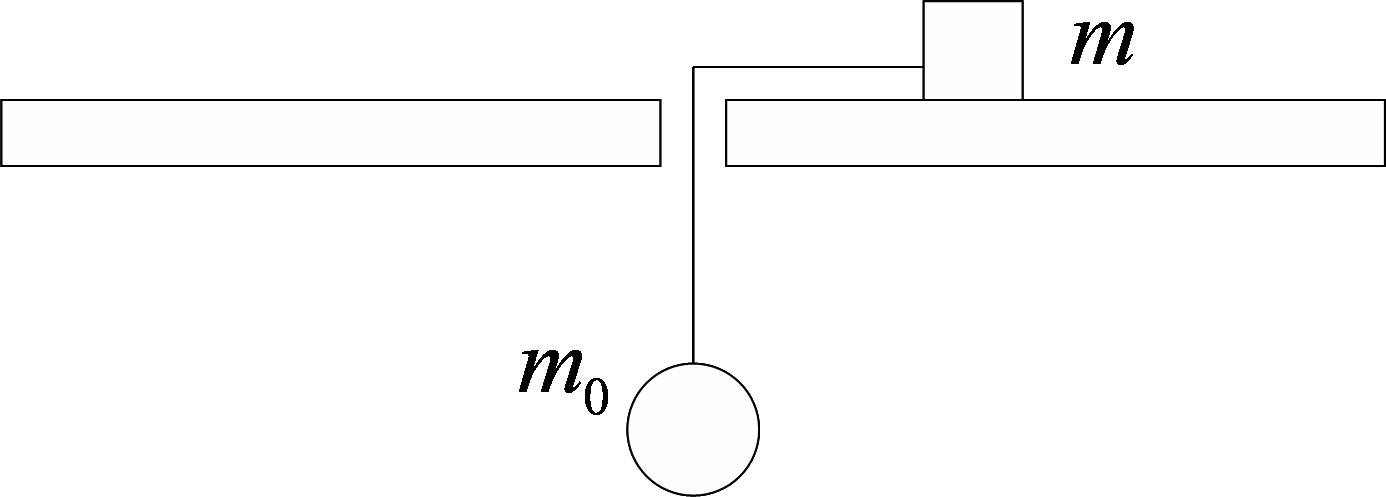
\includegraphics[width=0.4\textwidth, angle=0]{dyn/exercises/massa_op_tafel}
\end{center}
\end{figure}
\begin{enumerate}
\item Welke kracht levert de middelpuntzoekende kracht?
\item Kan voor cirkelbewegingen met een verschillende straal de
middelpuntzoekende kracht veranderen van grootte?
\item Hoe heb je proefondervindelijk geconstateerd dat de frequentie
voor verschillende stralen verschillend is?
\end{enumerate}

\end{exercise}

\begin{exercise} Een blokje op een wrijvingsloze tafel beschrijft een ECB met straal $r$ en snelheid $v$ doordat het vastgemaakt is aan een koordje dat door een gaatje in de tafel gaat en waaraan een massa is verbonden die door de zwaartekracht naar beneden wordt getrokken. Als de straal 2 maal groter wordt, hoeveel maal groter wordt dan de snelheid?
\begin{figure}[h]
\begin{center}
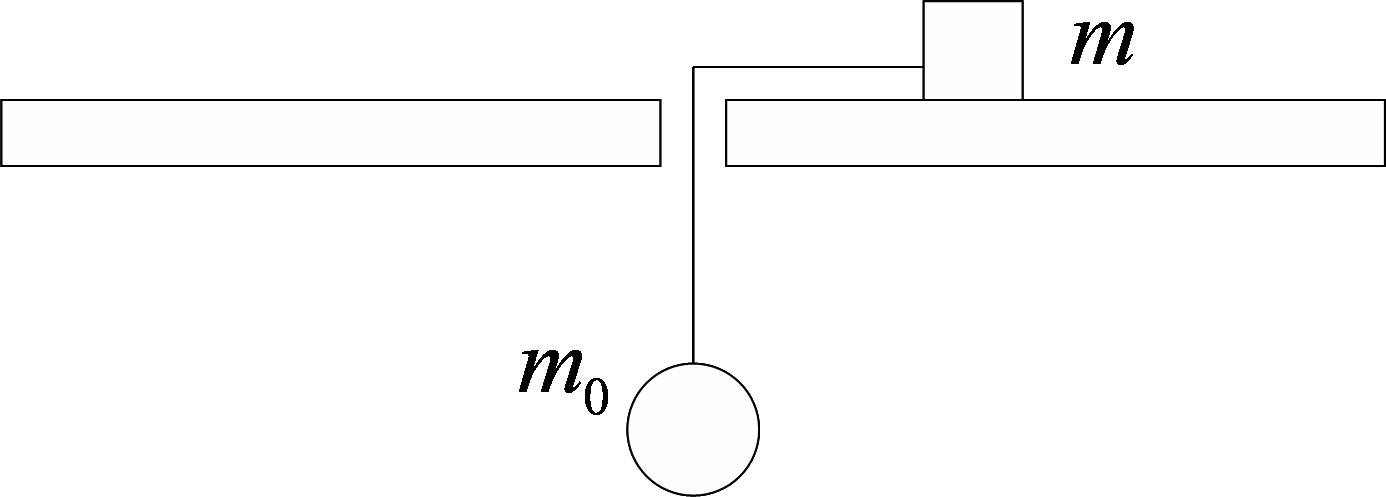
\includegraphics[width=0.4\textwidth, angle=0]{dyn/exercises/massa_op_tafel}
\end{center}
\end{figure}

\end{exercise}

\begin{exercise} Een blokje op een wrijvingsloze tafel beschrijft een ECB met frequentie $f$ en snelheid $v$ doordat het
vastgemaakt is aan een koordje dat door een gaatje in de tafel gaat en waaraan een massa is verbonden die door de zwaartekracht naar beneden wordt getrokken. Hoeveel maal groter is de snelheid van het blokje als het met een tweemaal zo grote frequentie ronddraait? Toon je antwoord aan.
\begin{figure}[!h]
\begin{center}
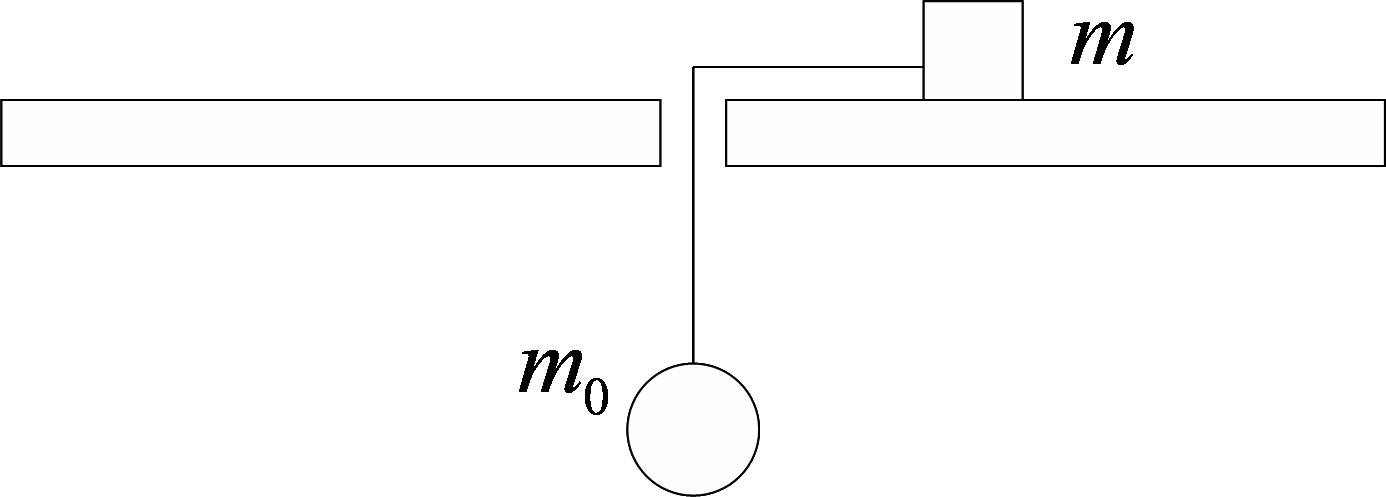
\includegraphics[width=0.4\textwidth, angle=0]{dyn/exercises/massa_op_tafel}
\end{center}
\end{figure}



\end{exercise}

\begin{exercise} Twee treinen met dezelfde massa nemen een bocht met een even grote straal. De snelheden zijn respectievelijk $60~\rm km/h$ en
$180~\rm km/h$ in de bocht.
\begin{enumerate}
\item \textit{Wat} levert de middelpuntzoekende kracht? Op
\textit{wat}?
\item Hoe verhouden de grootten van de middelpuntzoekende kracht zich?
\end{enumerate}


\end{exercise}

\end{document}